\documentclass{article}
\usepackage{fancyhdr}
\usepackage{graphicx}
\usepackage{hyperref}
\usepackage{booktabs}
\usepackage{array}
\usepackage{amsmath}
\usepackage[table]{xcolor}
\usepackage{xcolor}
\usepackage{longtable}
\usepackage[a4paper, margin=1in]{geometry}
\usepackage{caption}
\usepackage{ulem}















\pagestyle{fancy}
\fancyhead[L]{Defense Report : \textit{An Era of the Seas}}
\fancyfoot[L]{Dream Chasers}
\fancyfoot[C]{
    \begin{minipage}{1.5cm}
        \centering
        
\includegraphics[width=1cm]{logo.png}
    \end{minipage}
}
\fancyfoot[R]{\thepage}

\renewcommand{\footrulewidth}{0.1pt}
\renewcommand{\sectionmark}[1]{}
\renewcommand{\subsectionmark}[1]{}
\renewcommand{\contentsname}{}

\definecolor{lightblue}{HTML}{55FFFF}
\definecolor{pastelblue}{HTML}{097CA5}















\title{\textbf{Defense Report}\\
\textbf{\textit{An Era of the Seas}}}
\author{%
    \begin{minipage}[c]{\textwidth}
        \centering
        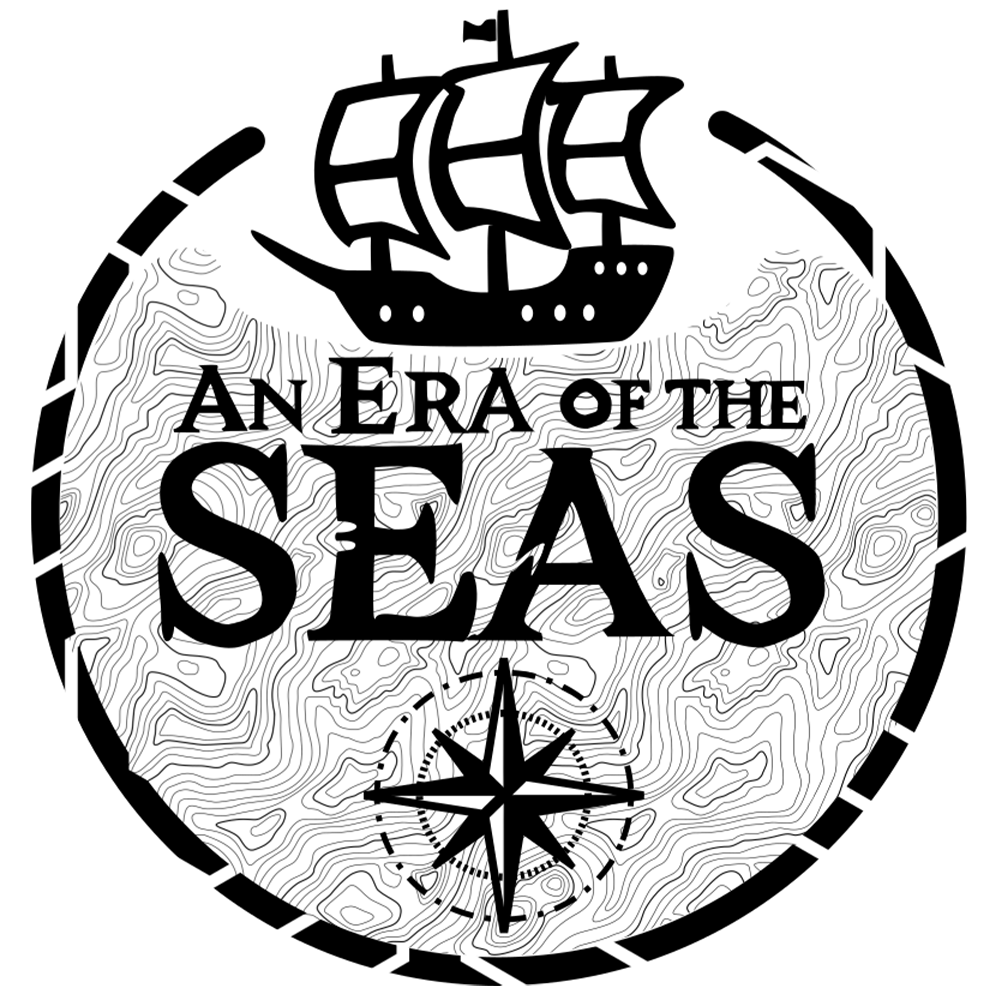
\includegraphics[width=3.5in]{AEotS Logo.png} \\
        \vspace{2cm}
        
\includegraphics[width=4in]{logo text.png}
    \end{minipage}
}
\date{}















\begin{document}

\maketitle

\vfill
\begin{center}
    \textbf{Lin Jérôme}\\
    \textbf{Ben Abdallah Achref}\\
    \textbf{Bruno Ethan}\\
    \textbf{Devin Joseph}\\
    \textbf{Class : A1}
\end{center}













\newpage
\thispagestyle{empty}
\addtocounter{page}{-1}
\null















\newpage
\section*{Introduction}\hfill

The project \textit{An Era of the Seas} stands out for its ambition to create a captivating maritime world where adventure and exploration lie at the heart of the gaming experience. Developed by the passionate team of \textbf{Dream Chasers}, this visual novel invites players to immerse themselves in the fascinating universe of sailing, through epic quests and strategic challenges.\\

\textit{An Era of the Seas} places players in the shoes of a captain who must traverse uncharted islands, confront formidable foes, and rebuild a family legacy. While navigating the Shattered Seas, players will discover a living, evolving environment designed to bring new life to every exploration. The realistic navigation system, ship upgrades, and crew management are all elements that enrich the experience while immersing the player in an authentic and intriguing world.\\

Through this project, \textbf{Dream Chasers} aims to deliver a complete and immersive gaming experience, combining technological innovation with narrative depth. The team strives to push the boundaries of video game development to offer a unique adventure, rich in discovery and strategy, that will captivate fans of exploration and piracy games.

\newpage
\subsection*{Summary}
\tableofcontents















\newpage
\section{Origin and nature of the Project}
\subsection{Origin}\hfill

The project for the game \textit{An Era of the Seas} stems from a shared interest among team members in video games and software development. It involves combining knowledge in computer science and video game development to create a captivating experience. This project is an opportunity to put acquired knowledge into practice by creating a tangible product.\\

Developing a game is an opportunity to acquire skills in various fields, from programming to graphic design, as well as sound production. Each member can contribute their unique skills, enriching the collective experience.\\

The rise of the video game industry and its growing importance in various domains such as education and entertainment also influenced the decision to create a game. It is an opportunity to immerse ourselves in the dynamic and ever-evolving video game sector.





\subsection{Game Information} 
\subsubsection{Beginning and Story of the Main Character}\hfill

\textit{An Era of the Seas} is a game where the maritime environment plays a central role. Players will embody the son of a great and powerful merchant who wielded significant influence and control over the seas. One day, he receives a letter informing him that his father perished during a mysterious expedition. Determined to uncover the truth, he begins his journey as a captain, aiming not only to restore his father's legacy but also to discover what truly happened.\\

As he explores the diversity of islands, he embarks on a voyage to become a great hero, just as his father was, while seeking answers to his own questions.



\subsubsection{Player Objectives}\hfill

Players will navigate and explore the islands of the Shattered Seas. To begin this adventure, the captain starts with nothing more than a small wooden boat he found on the shore. He must also explore eight different islands. Players will begin on the first island, where they will discover the main features, functionalities, and backstory of the son of the great merchant. Here, they will uncover the path to achieving the captain's ultimate goal.\\

The captain must travel to and reach each island to recover his father's scattered treasures and take control of the Shattered Seas. After exploring the first seven islands, the captain will finally be able to complete his journey on the last island, where the most challenging obstacles and trials await.



\subsubsection{Game Features}\hfill

This game offers unique features tied to its environment.

\paragraph{Main Quest}\hfill

This game is story-driven. Players will experience the captain's tale and be fully immersed in the game's maritime universe. Through the main quest, players will follow the captain's journey.

\paragraph{Side Quests}\hfill

While the main quest revolves around the captain's primary story, there are also secondary stories that unfold during his adventure across the seas and islands. These side quests can help players understand specific features and provide generous rewards. They involve completing tasks, deliveries, battles against specific enemies, or assisting residents of the Shattered Seas.

\paragraph{Immersive Navigation System}\hfill

The ship uses either wind or oars for navigation, depending on the ship's level and the crew's capabilities. This means starting with oars for lower-level ships, then progressing to harnessing the wind's direction, adjusting sails, and using the rudder for higher-level ships. To help the captain locate himself and chart a course to a specific destination, he will use a map and a compass.

\paragraph{Ship Maintenance and Upgrades}\hfill

The player's ship can be upgraded as they progress through the main quest. When the ship is damaged, the player must repair it using materials to continue navigating the seas. They can purchase a basic ship from a vendor and enhance it with specific materials.

\paragraph{Crew Members}\hfill

Since the player assumes the role of a captain navigating the seas, they have their own crew. This crew consists of various members with diverse tasks who have been carefully recruited from towns and quests to assist the captain on his journey. Each member has specific stats. Therefore, it is advisable to assign them to the appropriate tasks that will benefit the captain's journey. For example, some crew members are better suited to handle the oars, while others are more adept at exploration.

\paragraph{Weapons}\hfill

To fight against enemies, the player has the option to use swords and rifles. Weapons can be found in treasure chests, but these are common and low-powered. It is recommended to purchase weapons from merchants in the towns to acquire those with better stats and deal more damage.

\paragraph{Stigmata (Player Upgrades)}\hfill

Stigmata (Stigma in the singular) are marks inscribed on the hand with the help of a mage located in the towns. These marks enhance the player's abilities (speed, attack, etc.). They can be obtained by collecting them in treasure chests or by purchasing them from the mage. The mages have invested significant time and effort into creating the Stigmata. As a result, Stigmata sold by mages are much more effective and powerful than those found in nature. Therefore, buying Stigmata from a mage provides significantly higher stats than those found in treasure chests. Of course, this quality comes at a cost, as these Stigmata are far more expensive than those discovered in nature.

\paragraph{Treasure Chest}\hfill

To obtain resources and coins, treasure chests can be discovered on the islands and in areas guarded by enemies. These chests contain coins, weapons, Stigmata, and items to improve the ship, weapons, and Stigmata. These treasures help the captain build wealth, and since money means power in the Shattered Seas, it allows him to increase his influence over the seas.

\paragraph{Towns}\hfill

Each island has its own town, where various types of merchants can be found:
\begin{itemize}
    \item \textbf{Boat and Ship Makers:} They offer their exquisite creations, from small boats to massive ships. Depending on the island, these dealers provide better hulls and ship upgrades.
    \item \textbf{Weapon Makers:} They sell high-quality swords and rifles to face enemies.
    \item \textbf{Mages:} They use their mystical magic to inscribe a Stigma that the captain owns or has purchased. They also sell their own more powerful Stigmata.
    \item \textbf{Food Vendors:} They sell delicious food to the locals and adventurers, ensuring they don't run out of energy or starve to death.
\end{itemize}

\paragraph{Combat (PvE)}\hfill

In this adventure, the captain's journey is far from peaceful; he will encounter various enemies, both on the islands and across the seas. To defend himself and attack enemies, weapons, Stigmata, and the crew will be useful in battle. As with the seas, the ship can also attack, and the crew members are crucial in this regard. Therefore, the stats of weapons, Stigmata, the crew, and the ship are essential for dealing damage and withstanding enemy attacks.

\paragraph{Multiplayer}\hfill

This game features a multiplayer mode where players can choose a class and play according to it. In this mode, no advantages related to progress or items from the single-player mode are granted to the player.

\paragraph{Fishing}\hfill

A fun mechanic allowing the player to catch fish, which are useful for food and treasures like coins and resources. This is possible with a fishing rod that the captain possesses from the start of the game, and it can be used in large bodies of water such as lakes and oceans.





\subsection{Tools}
\subsubsection{Team Management Tools}\hfill

To communicate effectively on various aspects of game development among team members, it is crucial to have a dedicated tool. In this regard, a Discord server is particularly useful. It allows the team to easily communicate and organize discussions into different channels based on specific development topics.\\

Additionally, task management is essential for keeping the project on track and monitoring progress. A to-do list can be very helpful in this area, providing a clear overview of tasks to be completed. Microsoft To Do is an excellent solution for this. Tasks can be assigned to a team member, and a deadline can be set for each task. This allows team members to be aware of what needs to be done, the deadlines, and helps maintain their productivity.



\subsubsection{Game Development Tools}\hfill

Dream Chasers uses GitHub to work efficiently as a group on the project. It allows the team to track changes made to the game's code, ensuring that everyone is working on the latest version without overwriting others' work.\\

The game is coded in C\# (Csharp) for several reasons. C\# is an object-oriented programming language, a useful feature for games, and C\# is also commonly used in game engines like Unity.\\

For the IDE (Integrated Development Environment), the team uses Rider by JetBrains because it offers various advantages. It is specifically designed for .NET development (dotnet). Here, the team uses .NET Core 7 to develop the game. Rider's debugging tool is very powerful, making it easier to identify issues in the code through step-by-step debugging and variable monitoring. Additionally, Rider provides a Unity editor and is generally faster than other IDEs like Visual Studio.\\

The game engine used is Unity, as mentioned earlier, for many reasons. It provides an accessible user interface that simplifies project management for developers. With Unity, the game can be supported on multiple platforms, meaning it will run smoothly whether the player is using Windows, macOS, or Linux. It offers a variety of tools and features for the game's 3D environment, including an integrated physics engine.
















\newpage
\section{Study Objective}
\subsection{Interests and Objectives}\hfill

The main objective of the project is to create an immersive gaming experience, with a captivating story and engaging mechanics. Through this project, the team members will be able to apply the knowledge and concepts they have learned in a real and creative context. The game development process allows the team to overcome technical challenges and encourages them to develop practical problem-solving skills.





\subsection{Shared Benefits}\hfill

This project offers numerous benefits for teamwork.

Working with others fosters effective communication between team members, a crucial skill in the professional world. Through frequent discussions, team members develop the ability to clearly express their ideas, listen to feedback, and adapt to different perspectives.\\

Moreover, teamwork encourages better coordination, with management of task dependencies. Each team member can specialize in certain tasks, such as programming, game design, and audio engineering, which enhances productivity and efficiency. Task division also allows the project to progress more quickly, as tasks can be completed simultaneously.\\

Finally, teamwork leads to more innovative and creative solutions. Brainstorming can generate a variety of ideas, resulting in more original and unique game concepts and mechanics.





\subsection{Individual Benefits}\hfill

There are also many personal benefits to participating in this type of project.\\

Game development primarily allows developers to master specific technologies. For example, team members can focus on different aspects of game creation, such as game logic, physics engine, 3D design and animation, sound design, and more.\\

Additionally, team members will inevitably encounter technical challenges, obstacles, and problems throughout the process. Problem-solving strengthens problem-solving abilities, which is a crucial skill in any computer science career. Overcoming these challenges also boosts confidence and helps members become more adaptable.\\

In a collaborative project, each member must take on responsibilities. They are accountable for the quality and timeliness of their work. This can enhance the sense of autonomy and ownership. They must ensure that their contributions meet the team's expectations and deadlines, which helps in gaining independence.\\

Participating in a group project requires good time management. This means learning to balance personal work with the needs of the group. Team members must plan and prioritize their tasks, ensuring they contribute to the progress of the project.\\

Finally, working in a group on a game project allows members to acquire technical communication skills. Members must clearly explain ideas, solutions, and complex code to others, ensuring that everyone understands. This ability to communicate technical details in an accessible way is a very useful skill, one that will be frequently required in the professional world.















\newpage
\section{Company}
\subsection{Dream Chasers}\hfill

The company is called \textbf{Dream Chasers}, a name that reflects the company's spirit, in pursuit of creating an experience that turns the wildest dreams into reality. The company believes that games are not just mere entertainment; they are a gateway to new worlds, adventures, and the realization of fantastic ideas. The company's name is a tribute to those who dream and those who wish to chase those dreams.





\subsection{Specificities}\hfill

Dream Chasers stands out for its ability to blend technical skills with artistic expression. The company is dedicated to developing games that engage players not only intellectually, but also emotionally. The team is made up of enthusiastic developers, designers, and storytellers who view game creation as a form of art, combining cutting-edge technology, rich narratives, and immersive environments.\\

Dream Chasers' distinctive methodology is characterized by meticulous attention to detail, covering everything from gameplay mechanics to evocative music that enhances each scene. The company aspires to create not just games, but deep experiences that leave a lasting impression on players, encouraging them to reflect on their journey long after completing the game.\\

Furthermore, Dream Chasers prioritizes collaboration and innovation within its company culture. An atmosphere is cultivated to allow creativity to thrive, providing each team member with the opportunity to influence the trajectory of projects. This spirit of collaboration fosters new perspectives and continuous experimentation, ensuring that every game developed is a unique adventure.





\subsection{Field of Activity}\hfill

Dream Chasers operates in the dynamic field of video game development, but its scope extends beyond conventional gaming. The main goal lies in creating narrative-driven adventure games while exploring opportunities in educational technologies and virtual reality experiences.\\

Dream Chasers' aim is to create games that both educate and entertain, using interactive storytelling to address important themes such as environmental awareness, historical narratives, and personal growth. The company recognizes the potential of video games as effective learning and development tools, committing to integrate these elements into its projects as it moves forward.





\subsection{About the Game and the Company}\hfill

With this game, Dream Chasers engages players by asking if they have ever wondered what pirates did in the distant past. Players can feel a sense of nostalgia for the history of sailing and plundering in the Caribbean. This is why the team works closely with the Nostalgic Pirates Association (NPA) to develop this game, which aims to offer a refreshing reminiscence of the atmosphere and piracy of the 18th-century Caribbean. It will bring to life all the captains who lived during that era. Nostalgic pirates are invited to ask themselves if there is a more fulfilling way of life than sharing a drink with friendly crewmates on deck. Together, they can breathe the salty sea air, discover enchanting and unexplored islands, sail the seven seas, and embark on the search for magnificent treasures.\\

At Dream Chasers, there is a genuine commitment to addressing the concerns of the nostalgic pirate spirits, which is why the company helps those who can no longer pursue their dreams to experience them through a visual novel with the game \textit{An Era of the Seas}, designed for dreamers of the seas.















\newpage
\section{Team}\hfill

For this game, it is crucial to include individuals with diverse talents and specialties in order to offer players the world of their dreams.

\subsection{Jérôme}\hfill





Always close to cities from a young age, Jérôme aspires to understand how peaceful the natural environment can be. He chooses his own path by exploring the video game industry and aims to fulfill his ambitions by creating imaginary worlds with others. In this project, he will lead the team in creating a magnificent maritime world. He is also responsible for setting up items, rewards, chests, weapons, boats, Stigmata statistics, and account management.





\subsection{Achref}\hfill

Passionate about geek culture since childhood, Achref shaped his character by playing video games and watching numerous anime. In addition to that, his experience in the vast world of programming led him into the game development field, with a focus on story-based and role-playing games.





\subsection{Ethan}\hfill

From childhood to the present day, Ethan has always sought to understand how the world around him worked and how one could interact with it. Creating an environment with its own physics and logic represents a perfect opportunity to develop his understanding. He will oversee the game environment, such as water simulation, weather, and physics.





\subsection{Joseph}\hfill

Raised in the seaside city of Le Havre, Joseph grew to love the ocean and wants to explore this theme with his teammates during this project. Having been sailing for a long time, he is primarily responsible for implementing the navigation system in the game. Joseph is in charge of setting up the wind, managing the sails, the location system, and everything related to the ocean and navigation.















\newpage
\section{Task Distribution}
\begin{table}[h]
    \centering
    \begin{tabular}{|>{\columncolor{pastelblue!60}}l|c|c|c|c|}
        \hline
        \rowcolor{pastelblue!60}
        \textbf{Tasks} & \textbf{Jérôme} & \textbf{Achref} & \textbf{Ethan} & \textbf{Joseph}\\
        \hline
        Menu \& UI & \cellcolor{blue}R &  & \cellcolor{cyan}S &\\
        \hline
        Water Simulation & & & \cellcolor{blue}R & \cellcolor{cyan}S\\
        \hline
        Weather Simulation & & \cellcolor{blue}R & \cellcolor{cyan}S &\\
        \hline
        Movements (boat, player...) & & & \cellcolor{cyan}S & \cellcolor{blue}R\\
        \hline
        AI Movements (enemies, movements, attacks) & & \cellcolor{blue}R & & \cellcolor{cyan}S\\
        \hline
        Map & \cellcolor{cyan}S & & \cellcolor{blue}R &\\
        \hline
        Localization System (map, compass...) & & \cellcolor{cyan}S & & \cellcolor{blue}R\\
        \hline
        Item Statistics & \cellcolor{blue}R & & & \cellcolor{cyan}S\\
        \hline
        Fishing System & \cellcolor{cyan}S & \cellcolor{blue}R & &\\
        \hline
        Hunger System & & \cellcolor{cyan}S & \cellcolor{blue}R &\\
        \hline
        Network & \cellcolor{blue}R & \cellcolor{cyan}S & &\\
        \hline
        Multiplayer & \cellcolor{cyan}S & & & \cellcolor{blue}R\\
        \hline
        Story (Lore) & & & \cellcolor{cyan}S & \cellcolor{blue}R\\
        \hline
        Quests & & \cellcolor{cyan}S & \cellcolor{blue}R &\\
        \hline
        Website & & \cellcolor{blue}R & & \cellcolor{cyan}S\\
        \hline
        Entity Design & & \cellcolor{blue}R & \cellcolor{cyan}S &\\
        \hline
        Entity Animations & \cellcolor{cyan}S & & \cellcolor{blue}R &\\
        \hline
        SFX & \cellcolor{blue}R & & & \cellcolor{cyan}S\\
        \hline
        Music & \cellcolor{blue}R & \cellcolor{cyan}S & &\\
        \hline
        Code Optimization & \cellcolor{blue}R & \cellcolor{blue}S & \cellcolor{blue}S & \cellcolor{blue}S\\
        \hline
        Language Correction & \cellcolor{cyan}S & & & \cellcolor{blue}R\\
        \hline
        Testing & \cellcolor{blue}R & \cellcolor{blue}R & \cellcolor{blue}R & \cellcolor{blue}R\\
        \hline
    \end{tabular}
\end{table}

\begin{itemize}
    \item \textcolor{blue}{R : Responsible}
    \item \textcolor{cyan}{S : Substitute}
\end{itemize}















\newpage
\section{Progress and Planning}
\begin{longtable}{|>{\columncolor{pastelblue!60}}l|l|c|c|c|}
    \hline
    \rowcolor{pastelblue!60}
    \textbf{Deadline} & \textbf{Tasks} & \textbf{Progress} & \textbf{Responsible} & \textbf{Substitute}\\
    \hline
    27/10/2024 & Item Statistics & 25\% & Jérôme & Joseph\\
    \hline
    \multicolumn{5}{|c|}{\cellcolor{pastelblue!60}\textbf{B1 Exams (28-31/10/2024)}}\\
    \hline
    03/11/2024 & Map & 80\% & Ethan & Jérôme\\
    \hline
    10/11/2024 & Water Simulation & 50\% & Ethan & Joseph\\
    \hline
    10/11/2024 & Item Statistics & 50\% & Jérôme & Joseph\\
    \hline
    10/11/2024 & Item Improvements & 25\% & Jérôme & Joseph\\
    \hline
    10/11/2024 & Website & 80\% & Achref & Joseph\\
    \hline
    17/11/2024 & Main Menu & 40\% & Jérôme & Ethan\\
    \hline
    24/11/2024 & Main Menu & 80\% & Jérôme & Ethan\\
    \hline
    24/11/2024 & Localization System & 80\% & Joseph & Achref\\
    \hline
    01/12/2024 & Player Movements & 50\% & Joseph & Ethan\\
    \hline
    08/12/2024 & Player UI & 25\% & Jérôme & Ethan\\
    \hline
    15/12/2024 & Localization System & 100\% & Joseph & Achref\\
    \hline
    22/12/2024 & Player UI & 50\% & Jérôme & Ethan\\
    \hline
    22/12/2024 & Player Movements & 80\% & Joseph & Ethan\\
    \hline
    22/12/2024 & SFX & 20\% & Jérôme & Joseph\\
    \hline
    29/12/2024 & Entity Animations & 10\% & Ethan & Jérôme\\
    \hline
    28/12/2024 & Entity/AI Movements & 20\% & Achref & Joseph\\
    \hline
    29/12/2025 & Map & 100\% & Ethan & Jérôme\\
    \hline
    29/12/2024 & Boat Movements & 50\% & Joseph & Ethan\\
    \hline
    05/01/2025 & Entity Design & 25\% & Achref & Ethan\\
    \hline
    05/01/2025 & Boat Movements & 80\% & Joseph & Ethan\\
    \hline
    05/01/2025 & Weather Simulation & 50\% & Achref & Ethan\\
    \hline
    05/01/2025 & Water Simulation & 80\% & Ethan & Joseph\\
    \hline
    \multicolumn{5}{|c|}{\cellcolor{pastelblue!60}\textbf{B2 Exams (6-10/01/2025)}}\\
    \hline
    12/01/2025 & Story & 40\% & Joseph & Ethan\\
    \hline
    12/01/2025 & Main Quest & 40\% & Ethan & Achref\\
    \hline
    \multicolumn{5}{|c|}{\cellcolor{pastelblue!60}\textbf{First Technical Defense (13-17/01/2025)}} \\
    \hline
    12/01/2025 & Website & 100\% & Achref & Joseph\\
    \hline
    19/01/2025 & Player UI & 100\% & Jérôme & Ethan\\
    \hline
    26/01/2025 & Item Statistics & 100\% & Jérôme & Joseph\\
    \hline
    02/02/2025 & SFX & 40\% & Jérôme & Joseph\\
    \hline
    02/02/2025 & Entity/AI Movements & 50\% & Achref & Joseph\\
    \hline
    02/02/2025 & Entity Design & 50\% & Achref & Ethan\\
    \hline
    02/02/2025 & Main Quest & 75\% & Ethan & Achref\\
    \hline
    09/02/2025 & Weather Simulation & 100\% & Achref & Ethan\\
    \hline
    16/02/2025 & Entity Animations & 50\% & Ethan & Jérôme\\
    \hline
    02/03/2025 & Entity/AI Movements & 80\% & Achref & Joseph\\
    \hline
    02/03/2025 & Entity Design & 80\% & Achref & Ethan\\
    \hline
    02/03/2025 & SFX & 60\% & Jérôme & Joseph\\
    \hline
    \multicolumn{5}{|c|}{\cellcolor{pastelblue!60}\textbf{B3 Exams (03-07/03/2025)}}\\
    \hline
    10/03/2025 & Main Quest & 100\% & Ethan & Achref\\
    \hline
    10/03/2025 & Story & 80\%\ & Joseph & Ethan\\
    \hline
    \multicolumn{5}{|c|}{\cellcolor{pastelblue!60}\textbf{Second Technical Defense (10-14/03/2025)}} \\
    \hline
    30/03/2025 & Fishing System & 100\% & Achref & Jérôme\\
    \hline
    30/03/2025 & Hunger System & 100\% & Ethan & Achref\\
    \hline
    20/04/2025 & Entity/AI Movements & 100\% & Achref & Joseph\\
    \hline
    04/05/2025 & Entity Animations & 100\% & Ethan & Jérôme\\
    \hline
    25/05/2025 & Story & 100\% & Joseph & Ethan\\
    \hline
    \multicolumn{5}{|c|}{\cellcolor{pastelblue!60}\textbf{Final Technical Defense (26-30/05/2025)}}\\
    \hline
\end{longtable}















\newpage
\section{Technical Specifications}
\begin{itemize}
    \item Group Name: Dream Chasers
    \item Project Name: \textit{An Era of the Seas}
\end{itemize}





\begin{longtable}{|l|l|l|c|}
    \caption*{\textbf{\uline{Names of the Members}}}\\
    \hline
    \rowcolor{pastelblue!60}
    Last Name & First Name & Login & Class \\
    \hline
    Ben Abdallah & Achref & achref.ben-abdallah & A1 \\
    \hline
    Bruno & Ethan & ethan.bruno & A1 \\
    \hline
    Devin & Joseph & joseph.devin & A1 \\
    \hline
    Lin & Jérôme & jerome.lin & A1 \\
    \hline
\end{longtable}





\begin{longtable}{|c|c|c|c|c|}
    \caption*{\textbf{\uline{Game Types}}}\\
    \hline
    \cellcolor{lightblue}Action/Adventure & Battle Royale & Beat them up & Combat & Simulation \\
    \hline
    \cellcolor{lightblue}FPS & MMORPG & MOBA & Party Games & Survival Horror \\
    \hline
    Platformer & Puzzles & Strategy & Rogue-like & TPS \\
    \hline
    \cellcolor{lightblue}RPG & RTS & Sandbox & Shoot them up & Racing \\
    \hline
    Other: & \multicolumn{4}{|c|}{} \\
    \hline
\end{longtable}





\begin{longtable}{|>{\columncolor{pastelblue!60}}l|l|l|l|l|}
    \caption*{\textbf{\uline{Features}}}\\
    \hline
    \multicolumn{5}{|c|}{\cellcolor{pastelblue!60}\textbf{General Game Features}}\\
    \hline
    AI & \cellcolor{lightblue}Wander & \cellcolor{lightblue}Attack & \cellcolor{lightblue}Escape & "Path Finder"\\
    \hline
    Multiplayer & \cellcolor{lightblue}Cooperative & Battle (2-4) & \multicolumn{2}{|l|}{Massive}\\
    \hline
    Network & P2P & Lan & \multicolumn{2}{|l|}{\cellcolor{lightblue}Online}\\
    \hline
    \multicolumn{5}{|c|}{\cellcolor{pastelblue!60}\textbf{Graphic Features}}\\
    \hline
    Dimension & 2D & \cellcolor{lightblue}3D & Other: &\\
    \hline
    Specifics & Stereoscopy & AR & \multicolumn{2}{|l|}{VR}\\
    \hline
    Graphics & \cellcolor{lightblue}Custom & Custom & \multicolumn{2}{|l|}{\cellcolor{lightblue}Existing}\\
    \hline
    Details: & \multicolumn{4}{|c|}{}\\
    \hline
    \multicolumn{5}{|c|}{\cellcolor{pastelblue!60}\textbf{Sound Features}}\\
    \hline
    Music & Custom & Custom & \multicolumn{2}{|l|}{\cellcolor{lightblue}Existing}\\
    \hline
    FX & Custom & \cellcolor{lightblue}Custom & \multicolumn{2}{|l|}{Existing}\\
    \hline
    Details: & \multicolumn{4}{|c|}{Musical theme focused on a maritime universe}\\
    \hline
    \multicolumn{5}{|c|}{\cellcolor{pastelblue!60}\textbf{Other Features}}\\
    \hline
    Website & Custom & \cellcolor{lightblue}Custom & \multicolumn{2}{|l|}{Prefabricated}\\
    \hline
\end{longtable}







\begin{figure}[h]
    \caption*{\textbf{\uline{GANTT Chart}}}
    \centering
    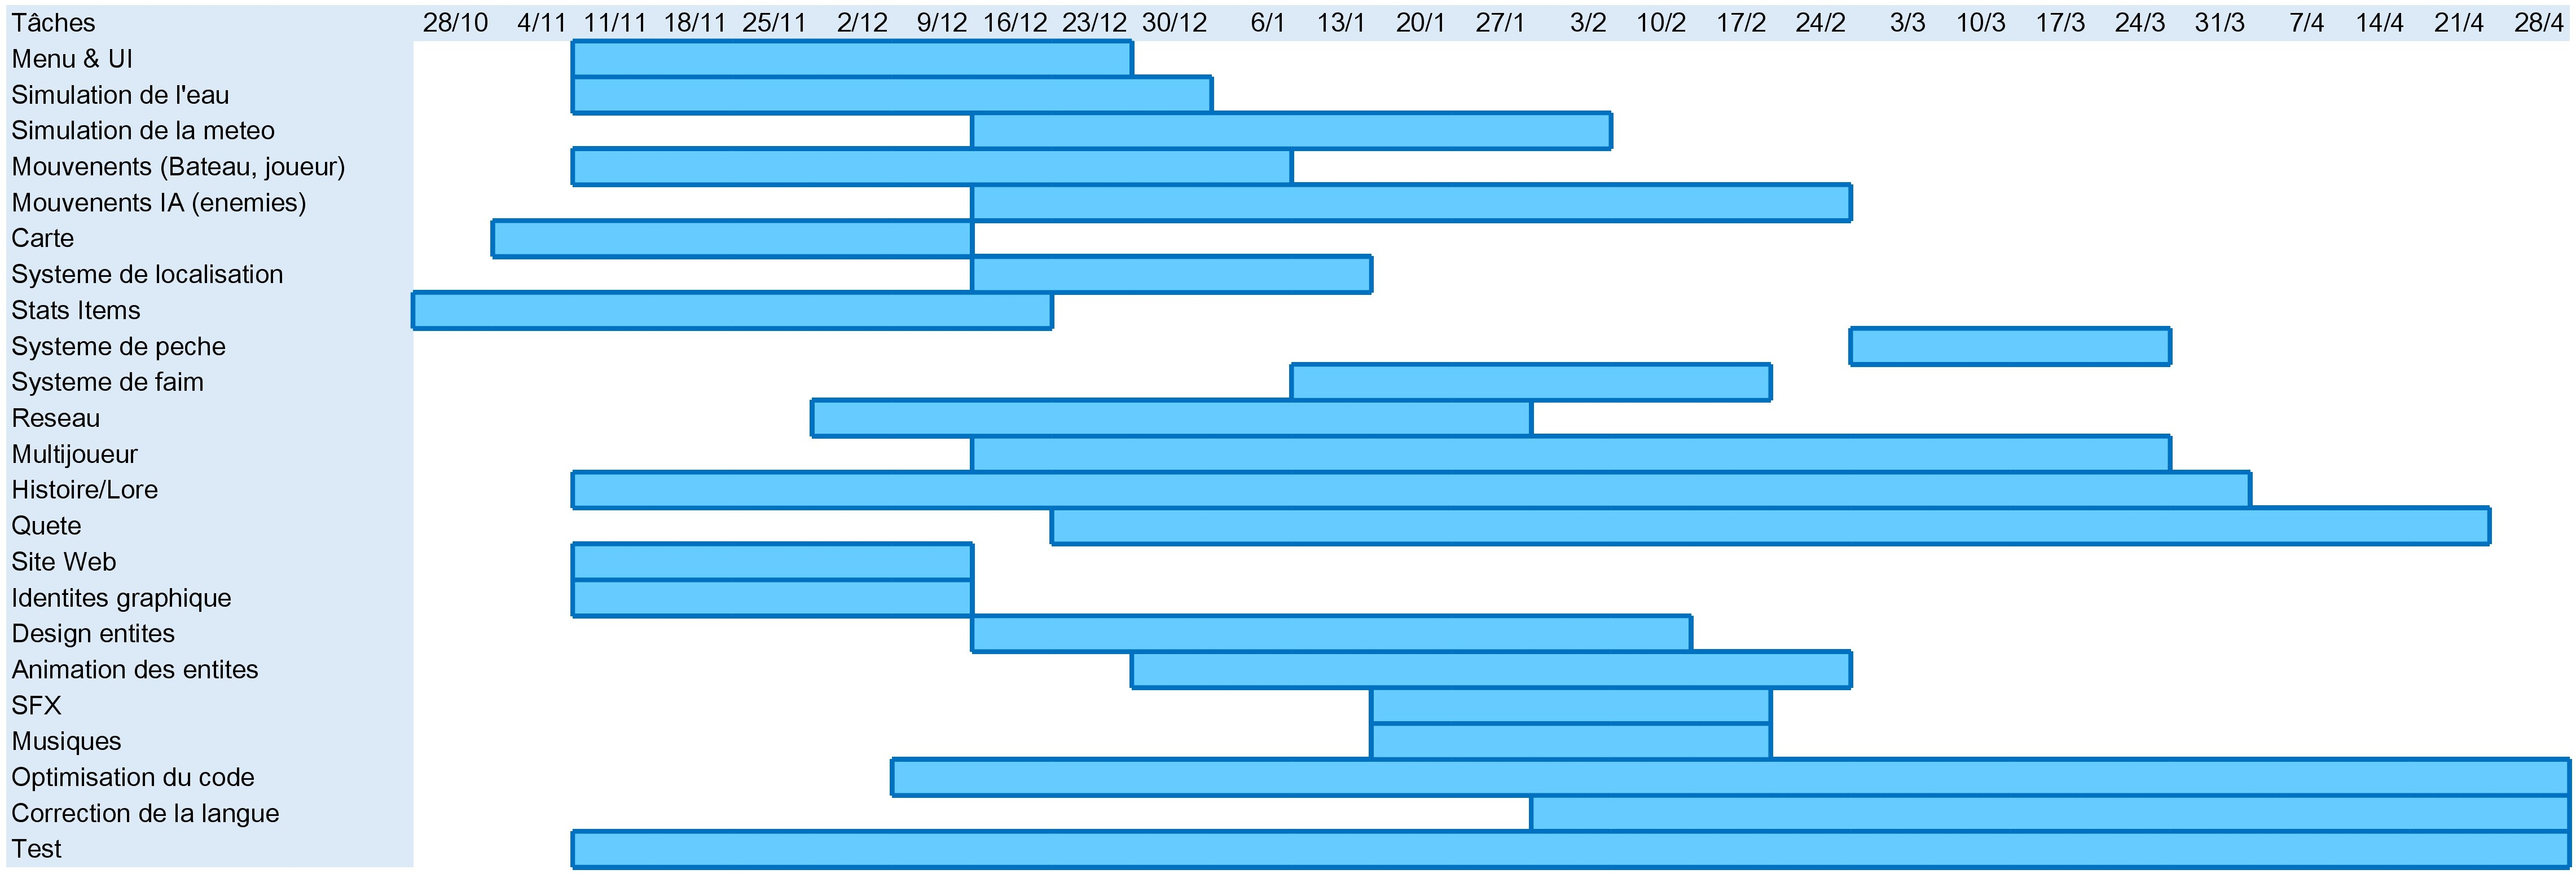
\includegraphics[angle=90, width=4.2in]{gant.png}
    \label{fig:my_image}
\end{figure}















\clearpage
\section{Development Narrative}
\subsection{Jérôme}
\subsubsection{Implementation of Objects in the Game}\hfill

The development of the game began with a crucial phase: listing all the objects that would appear in the game. These objects were highly diverse, ranging from weapons like swords and firearms to stigmata, ships, crew members, and various materials such as coins, drops of pure water, wood, and steel. One of the most challenging aspects of this initial phase was coming up with original and captivating names for each of these items. This required a significant amount of creativity and inspiration, which led me to spend a considerable amount of time browsing the internet to gather ideas and fuel my imagination. The search for fitting names took longer than anticipated, but in the end, it was very rewarding to see everything come together.\\

Once this initial challenge was overcome, I proceeded to structure this information in a JSON file. Fortunately, I was already familiar with working with JSON files, which made this part of the task relatively simple and fast. Having a well-structured format in place allowed me to move forward with confidence.\\

Next, I faced a more complex challenge: creating an Excel document to define the player's base statistics depending on their level, knowing that the maximum level in the game would be 100. It was important to also determine the materials required to upgrade the player's level. Finding the right formulas for this purpose was quite a puzzle. I explored different models of exponential and linear growth, and I worked hard to define precise statistics for both level 1 and level 100. Even though I was quite comfortable with Excel, this step still required extensive online research, as the formulas I needed were quite specific and not immediately available in tutorials.\\

After finalizing the player's statistics, I moved on to defining the statistics for each type of item. Armed with the formulas I had established earlier, this step turned out to be quicker, although repetitive. However, I found myself adjusting the stats for levels 1 and 100 on several occasions to maintain a consistent balance with the player's stats. Ensuring these numbers aligned was critical, as any discrepancy would have a significant impact on the game's overall difficulty and player experience.\\

Once all the necessary data had been compiled and organized, it was time to export it from Excel files (.xlsx) to CSV files (.csv). This conversion was crucial, as it would allow me to work with the data in C\# and eventually load it into Unity.\\

Then came a pivotal phase in the development: writing scripts to integrate the game objects into Unity. This task involved handling both the JSON and CSV files, and I discovered and utilized two highly popular libraries to manage this process: Newtonsoft.Json for JSON files and CsvHelper for CSV files. The beauty of these libraries was their widespread use, which made finding resources, tutorials, and documentation easy.\\

To fully grasp how to load the data correctly, I studied the documentation of these libraries in detail and watched several explanatory videos on YouTube. Handling JSON files proved to be a bit tricky, as the formatting and parsing were more complex than I initially thought, while working with CSV files was a bit more intuitive. Even so, there were several hurdles along the way, and it took time to get everything working perfectly.\\

Once the loading functions were set up, the next step was to implement them in Unity using MonoBehaviour scripts. This opened the door to several additional challenges. One of the primary issues I encountered was how to efficiently share data between the scripts. Once I figured out the best approach for communication, another problem arose: the scripts weren't being executed in the right order. To solve this, I had to modify the script execution order in Unity's game profile, which was a bit tricky but essential for everything to work as expected.\\

Once these loading issues were sorted out and everything was functioning properly, I could finally tackle another critical step: managing the player's data.\\

Initially, I had planned to use Firebase Realtime Database to store player data. However, I quickly realized that it would be impossible to integrate the necessary libraries, available via NuGet, into a Unity project. Facing this limitation, I decided to go with a local solution: saving player data in JSON files. This approach had already been suggested to me during my research on how to handle save data in Unity, so it seemed like a reliable and feasible option.\\

The JSON file needed to store several important elements: the player's position, level, and inventory. As for the inventory, I had already planned a logical structure: distinguishing between the items equipped by the player and those stored in their inventory. This distinction was key for the game mechanics, as equipped items would affect the player's stats, while stored items were simply available for use when needed.\\

With this structure in mind, I set out to write a script that would manage these data. The script needed to load the information from the JSON file and convert it into a usable C\# object. Once the data was loaded, it was necessary to recalculate the player's statistics based on various bonuses provided by the stigmata and the weapon they had equipped.\\

This phase was more intuitive than I had anticipated. Most of the research required had already been completed during previous steps, and I had written the scripts for loading the data for the game objects. Now, I simply had to apply this data to adjust the player's stats accordingly.\\

Although this part of the process was largely technical, it went smoothly. It was rewarding to see the system working as expected and to watch the player's stats dynamically change based on the items they equipped. This was one of those moments in the project when everything felt like it was falling into place.\\

This milestone represented a significant advancement in the game's development and brought me closer to realizing my final vision for the project. Each challenge overcome and every line of code written reinforced both my understanding and my enthusiasm for this game.



\subsubsection{Menu \& User Interface}\hfill

Before diving into Unity, I took the time to research and study how to create menus and user interfaces within the engine. I consulted several guides and watched multiple YouTube videos to understand the ins and outs of UI development. At first glance, this seemed relatively simple, but I knew I would need to pay close attention to how the buttons and other UI elements were presented. My primary goal was to create a clear, intuitive interface that would not disrupt the player's experience.

\paragraph{Designing the Main Menu}\hfill

I began by placing the buttons and designing the background for the main menu. Finding an appropriate background was surprisingly quick thanks to Unity's Asset Store. I discovered a set of images that fit perfectly with the maritime theme of my game, which helped set the tone for the menu's overall aesthetic.\\

However, finding pre-made buttons that suited my needs turned out to be more difficult. After searching through the available assets, I couldn't find any that matched my vision, so I decided to create my own. With my experience in photo manipulation, I designed custom buttons and selected a font that harmonized with the overall aesthetic of the game.\\

Integrating these buttons into Unity was a valuable learning experience. At first, I didn't understand how to replace the default Unity button sprites with my own designs. I simply tried to drag and drop my image files into the sprite area, but it didn't work. After some research, I learned that I needed to convert my image files into sprites before they could be used. Once I mastered this step, I was able to apply my custom creations and give the main menu a unique and immersive visual appearance.

\paragraph{Scripts for UI Navigation}\hfill

The next step was writing the scripts to handle interactions between the different menu elements. I needed to allow the user to switch between canvases or show and hide GameObjects depending on their actions. This part was relatively straightforward, thanks to a built-in function in Unity, and the research I had to do to understand how it worked was minimal.

\paragraph{Designing the Inventory Menu}\hfill

The real challenge with the user interface came when I started working on the inventory menu. This menu needed to dynamically display the items the player had acquired, which was a far more complex system than the main menu. Fortunately, I came across a video tutorial that explained exactly how to accomplish what I wanted. By following this tutorial step by step, I was able to understand the necessary processes and overcome the challenges without too much difficulty.\\

As I worked on this more complex inventory system, I had to ensure that the displayed items would be properly updated in real-time, based on what the player had in their inventory at any given moment. The solution required integrating a dynamic data-binding system where items could be added, removed, or updated as the player interacted with the game world. This meant creating an inventory system that could handle various types of objects, each with their own properties and associated visuals. As I developed this part, I had to consider how to visually represent these items in a way that would be easy for the player to understand, which included designing icons, organizing inventory slots, and allowing for efficient item sorting.\\

This stage of the development allowed me to explore a variety of Unity's UI components in depth, such as ScrollViews, Buttons, and TextMesh Pro for text formatting. It also required me to revisit some C\# programming concepts to ensure that the data was handled correctly and presented seamlessly within the game.\\

The process of creating the inventory menu was quite rewarding. Although it was a complex challenge, it was satisfying to see the system come together and function as intended. Each time I made an improvement or fixed an issue, the entire user experience became more polished and coherent, making the game much more enjoyable to navigate. This also provided me with the tools to build other menus in the future, using the same principles and structure I developed for the inventory.



\subsubsection{Organization}\hfill

From the very beginning of the project, I took the initiative to volunteer as the project manager, driven by my strong sense of organization and attention to detail. This responsibility allowed me to structure the development phases and guide my team toward achieving our final objective. Taking on this leadership role was a way for me to both contribute to the project's success and hone my organizational skills.

\paragraph{Defining Tasks and Creating a Schedule}\hfill

The first step was to define the different tasks that needed to be accomplished, which turned out to be relatively straightforward. Once the tasks were identified, the next challenge was to assign them among the team members and ensure that everyone agreed on the distribution. This involved understanding each member's strengths and weaknesses, and balancing the workload to avoid overburdening any one person while ensuring that all tasks were covered.\\

The real challenge came in creating a clear, visual schedule. Initially, I started with a simple table that followed the requirements of the specifications document, including the percentage of tasks assigned to each team member. While this table technically met the requirements, I soon realized that it lacked readability and was not optimal for tracking the project's progress in a comprehensive way. To make the schedule more accessible and understandable, I decided to create a Gantt chart, which would give a more visual and intuitive representation of the project's timeline. Thanks to Excel, creating this chart was quick and efficient, and it greatly enhanced communication and collaboration within the team. It allowed everyone to visualize the project's progress and deadlines, making it easier for us to adjust as needed.

\paragraph{Adjustments After the First Technical Specification}\hfill

After submitting the first technical specification document, I noticed some imbalances in the distribution of tasks. Some team members had taken on more responsibility than others, and this needed to be addressed in order to ensure a fair workload. I took the time to review the task distribution and made minor adjustments where necessary. I also consulted the rest of the team to validate these changes, ensuring that everyone was comfortable with the new assignments and that the workload was evenly spread.\\

This process of reviewing and revising the tasks was crucial to maintaining the project's momentum. Regular reassessments of the schedule allowed us to catch any potential issues before they became bigger problems and to make sure that no team member was left feeling overwhelmed or underutilized.

\paragraph{Attendance Issues}\hfill

Another organizational challenge arose when one of the team members failed to meet the deadlines for their assigned tasks. Just one week before the methodological defense, the 2D map and the game logo were still not completed. This was a critical situation, as these tasks were essential for the project's progress. Faced with this setback, I had no choice but to take over the creation of the 2D map myself to ensure the project didn't fall behind. Fortunately, the logo, which was being created by the team member, was eventually completed, albeit later than expected. Despite the delay, we were able to adapt and move forward without compromising the overall quality of the work.\\

This situation taught me a valuable lesson in flexibility and time management. Although it was frustrating to have to take on additional tasks, I was able to maintain focus on the bigger picture and ensure that the project continued to move forward. Additionally, I had to consider how to better monitor progress in the future to avoid such situations.

\paragraph{Departure of a Team Member Before the Defense}\hfill

The most significant challenge occurred the day before the methodological defense: one of the team members, Matteo Bollot, announced that he was leaving the institution. This sudden departure threw a wrench into our plans, as we now faced the issue of ensuring an equitable distribution of speaking time during the defense presentation. Matteo's departure left us with one less voice to represent the project, and this required a quick and coordinated response.\\

Thanks to the prompt reaction of the remaining members, we were able to quickly rearrange the speaking roles and adjust the presentation accordingly. We divided the speaking time equally among ourselves, and the presentation went ahead without any major issues. This unexpected change highlighted the importance of being adaptable and flexible, as unforeseen circumstances can often throw projects off course. In the end, the defense went smoothly, and we were able to present our work effectively.\\

After Matteo's departure, the team was reduced to four members. This shift required me to reassess the distribution of tasks to account for the additional workload now spread among fewer people. I took extra care to consult the remaining team members before finalizing these adjustments, as I wanted to ensure that no one felt overwhelmed by the added responsibility. Though each member now had a bit more work, I decided to stick to the original planning, hoping that everyone would continue to meet their commitments despite the changes. This phase of the project was a reminder of the importance of communication and collaboration, especially when dealing with unexpected setbacks.

\paragraph{Conclusion}\hfill

This experience as a project manager exposed me to various human and organizational challenges, but it also allowed me to strengthen my skills in group management. I learned the importance of maintaining a clear and realistic vision for the project while being flexible enough to adjust when necessary. While the challenges were significant, they were ultimately manageable due to the collaborative and proactive approach we adopted as a team. Despite the unexpected hurdles, the team remained cohesive, and we continue to make progress toward the completion of our video game. Through each difficulty, we became better at navigating the complexities of teamwork and project management, which will undoubtedly benefit us in future endeavors.



\subsubsection{Linking the player interface with the inventory}
\paragraph{Objective}\hfill

The primary goal of this phase was to establish a seamless connection between the game's UI and the player's inventory, ensuring that item management was both intuitive and efficient. This required careful implementation of item sprites, inventory interaction, item upgrading, and equipment management. A secondary objective was to create a robust system that could handle potential expansions, including additional items and functionalities in future updates.

\paragraph{Research and methods}\hfill

To begin, the game required a vast array of item images, including Stigmata, weapons, boats, coins, Pure Water Drops, steel, and wood. Gathering and researching appropriate visual assets for these elements took considerable time. After selecting the necessary images, they were configured as sprites in Unity and renamed to match their corresponding item names. This approach streamlined asset management and ensured consistency within the game's database.\\

To integrate these items into the inventory UI, object-oriented programming principles were applied. The game retrieves item data from CSV and JSON files, structured during the early development phases as part of the Items Stats Implementation. By leveraging this data-driven approach, item integration became a matter of efficient object manipulation within Unity, allowing for a scalable and flexible inventory system.

\paragraph{Implementation}\hfill

Players needed to be able to upgrade items and utilize materials such as Coins, Pure Water Drops, Steel, and Wood. This required the creation of an Upgrade Menu within the Player Interface. Implementing this feature was particularly challenging due to potential errors related to null variables when switching between different menus. Furthermore, to enhance accessibility, the Upgrade Menu had to be accessible from both the Inventory Menu and the Equipment Menu, adding another layer of complexity to its implementation.\\

Beyond inventory management, the Equipment Menu needed to facilitate the handling of equipped items. A crucial requirement was to enable seamless switching between items, leading to the development of a Switch Item Menu. After working through the complexities of the Upgrade Menu, item switching within the UI became more intuitive and easier to manage.\\

A major challenge arose when designing the interface for equipping crew members on the player's boat. The number of available crew slots varies based on the boat's level, meaning the Equipment Interface had to function similarly to the Inventory but with added complexity. Unlike the standard inventory, which operates with a single scroll view, the crew management interface required four separate scroll views to efficiently accommodate multiple crew members. The interface had to dynamically adjust based on the boat's level, ensuring that new crew slots became available as the boat upgraded.\\

After extensive testing and iterations, the crew management interface was fully operational, successfully integrating dynamic slot allocation and an intuitive UI layout. This achievement marked a significant milestone, ensuring that players could manage their crew efficiently while maintaining the immersive and interactive nature of the game's UI.

\paragraph{Conclusion}\hfill

The process of linking the UI with the player inventory and equipment system was both complex and rewarding. It required a combination of asset management, object-oriented programming, and UI design expertise. The most challenging aspects included managing seamless UI transitions, ensuring data integrity across menus, and implementing dynamic features such as crew slot allocation based on boat progression.\\

Despite the obstacles, careful planning, iterative problem-solving, and rigorous testing resulted in a polished and fully integrated inventory and equipment system. This not only enhances the player experience but also lays a strong foundation for potential future expansions, ensuring that the game remains engaging and adaptable to future content updates.



\subsubsection{Map design}
\paragraph{Objectives}\hfill

After repeatedly reminding my associate, who was responsible for the map, to push his work onto the Git repository, he finally submitted it. However, upon reviewing his submission, I realized that the work was incomplete—the island merely had the basic shape corresponding to the 2D map without any additional details or refinement. Recognizing the necessity of a properly developed environment, I decided to take over the task of building the first island, despite it not being my original responsibility. The map required various textures, such as grass, sand, and roads, to create a visually appealing and immersive environment. Additionally, there was a significant gap between the marine and terrestrial sections of the terrain.

\paragraph{Research and methods}\hfill

To address this, I reshaped the island's height to provide a more natural and seamless transition between land and water before applying the necessary textures to the terrain. Upon further examination, I noticed that the map was devoid of trees, villages, and other structural elements. Fortunately, before receiving my coworker's incomplete work, I had already conducted research on the Unity Asset Store and identified suitable 3D models for villages and marketplaces. With these assets readily available, I imported them into the project and strategically placed the prefabs to create a village, complete with a market and houses dispersed throughout the island. For vegetation, I utilized Unity's built-in terrain tools to populate the environment with trees, ensuring a natural and diverse landscape.

\paragraph{Implementation}\hfill

I reshaped the island's height to provide a more natural and seamless transition between the land and water before applying the necessary textures to the terrain. I imported suitable 3D models for villages and marketplaces from the Unity Asset Store and strategically placed them on the map. I populated the environment with trees using Unity's built-in terrain tools to ensure a diverse and realistic landscape.

\paragraph{Conclusion}\hfill

Stepping in to complete the first island's development demonstrated the importance of adaptability and problem-solving in game development. Ensuring a visually engaging and functional map was crucial for creating an immersive player experience.



\subsubsection{Boat and player movements review}
\paragraph{Objectives}\hfill

After reviewing the map, I decided to evaluate other core functionalities of the game, specifically the movement of both the player and the boat. Upon testing these mechanics, I found that while both movement systems were functional, the boat movement lacked precise control, particularly when the player needed to interact with specific objects on board. One of the main issues was the interaction system for key elements such as the Helm and the Capstan. Initially, two very similar scripts handled these interactions separately, but the player also needed to interact with additional objects, such as chests.

\paragraph{Research and methods}\hfill

To optimize the system and reduce redundancy, I merged these scripts into a unified Interactor Handler, streamlining the interaction process for all relevant objects. Another critical problem was that the player could fall off the boat while it was moving. To prevent this, I created a box of colliders to keep the player on board. However, these colliders initially blocked the player from entering the boat. To address this, I integrated the Interactor Handler, allowing the player to board and disembark smoothly by pressing 'E' to enter and 'X' to exit the boat.
Additionally, when the player switched to the Helm camera view, they needed to remain attached to the boat to prevent being ejected upon exiting Helm mode. This was resolved by ensuring that the player was properly parented to the boat while steering.

\paragraph{Implementation}\hfill

I merged the separate interaction scripts into a unified Interactor Handler, which optimized and streamlined the interaction process for all objects that the player could engage with. I created a box of colliders around the boat to prevent the player from falling off during movement, while ensuring that the colliders did not block the player from boarding the boat. This was achieved by integrating the Interactor Handler, which allowed the player to enter and exit the boat smoothly using the 'E' and 'X' keys. I also ensured that when the player switched to the Helm camera view, they were parented to the boat, preventing ejection upon exiting Helm mode.

\paragraph{Conclusion}\hfill

The refinement of movement mechanics and interaction systems was a crucial step in improving gameplay fluidity and player experience. By consolidating interaction scripts into a single handler, I eliminated redundancy and made the system more efficient. Implementing solutions to prevent the player from falling off the moving boat further enhanced gameplay realism and accessibility. These optimizations, combined with the map development and UI improvements, contributed to a more immersive and polished game experience. Through thorough testing and iteration, these features were successfully integrated, ensuring a stable and engaging gameplay foundation.



\subsubsection{Animations}
\paragraph{Objectives}\hfill

After verifying the movement system, I noticed that a crucial task had not been completed despite being planned. Taking the initiative, I decided to implement the player's animations myself, even though it was not originally assigned to me. The goal was to set up smooth and responsive animations for various player actions such as idle, running, walking, attacking, swimming, and death, and to ensure that these animations worked seamlessly with the movement system.

\paragraph{Research and methods}\hfill

Starting with basic concepts such as animations and skeletal structures, I researched animation techniques and followed three YouTube tutorials to build my understanding:
\begin{itemize}
    \item \url{https://youtu.be/2_Hn5ZsUIXM}
    \item \url{https://youtu.be/vApG8aYD5aI}
    \item \url{https://youtu.be/s5lRq6-BVcw}
\end{itemize}
I then downloaded all necessary animations from Mixamo (\url{https://www.mixamo.com}), including idle, running, walking, attacking, swimming, and death animations. With the knowledge gained from the tutorials, I successfully set up the Animator Controller. However, when testing it with the player model, the animations did not work. After further investigation, I discovered that the player's model lacked a skeleton. Initially, I attempted to create a skeleton using Unity's Rig menu, but after multiple failed attempts and additional research, I realized an alternative approach was necessary.\\

I decided to create a bone structure in Blender and then reimport the player model with the skeleton. Following the tutorial (\url{https://youtu.be/gdOaUv0_TC8}), I successfully rigged the character.

\paragraph{Implementation}\hfill

Once the bones were in place, I applied the Animator Controller to the model, and the animations worked correctly. The final step was scripting the transitions between animations based on player actions, such as running, attacking, swimming, and jumping. For the jump animation, special considerations were needed since the falling animation had to dynamically adjust based on factors like jumping from a high cliff. To refine the jumping mechanics, I followed this tutorial (\url{https://youtu.be/sJvWmFYSQFY}), and the implementation worked perfectly.

\paragraph{Conclusion}\hfill

The animation implementation was a critical enhancement to the player's experience. By setting up a proper skeleton and configuring the Animator Controller, the game now features smooth and responsive animations. The integration of movement transitions ensures a more immersive and dynamic gameplay experience, reinforcing the overall quality of the project.


\subsubsection{Player Texture}
\paragraph{Objectives}\hfill

After testing the animation, I noticed that the player could see his own texture through the first-person camera, such as his own leg, which created an unrealistic and immersion-breaking effect. The issue was that the player could see the inside of the 3D model's texture from their own perspective. The goal was to find a solution to hide the player's texture only from their own camera while ensuring that in a multiplayer context, other players' textures would still remain visible. This correction was essential to preserve immersion and realism during gameplay.

\paragraph{Research and methods}\hfill

In this case, with the current player model, I first attempted to change the material directly, but I quickly realized that there was no Mesh Renderer component visible in the Inspector for the 3D model in Unity. This prevented me from applying a new material directly to the original model. As a result, the only viable solution was to extract the albedo texture (the color texture) from the original .fbx model, recreate a material using this texture, and then apply it to a duplicate of the player model, this time with a Mesh Renderer in the Inspector to allow proper material management.\\

To extract the albedo texture, which was a .png file, I used Blender and followed the tutorial \url{https://youtu.be/wG6ON8wZYLc}. This process took quite some time, as it required careful handling to export the texture properly from the model and ensure its integrity for reuse in Unity.

\paragraph{Implementation}\hfill

Once the .png texture was successfully extracted, I imported it back into Unity and applied it to the duplicate player model that featured the required Mesh Renderer component. With the model now properly set up to receive materials, I created an invisible material. After quickly researching methods online, I developed a functional invisible material that worked perfectly when applied to the model, making the player's body entirely transparent from their own perspective.\\

To handle the switching between the visible and invisible materials, I wrote a simple script. This script toggled the materials depending on the active camera or gameplay state, ensuring that the player's model would become invisible from the first-person view while maintaining normal visibility for other players in multiplayer mode.

\paragraph{Conclusion}\hfill

Thanks to the successful extraction of the albedo texture and the creation of an invisible material, the player can now enjoy an immersive first-person experience without seeing parts of their own body breaking the visual continuity of the game. This implementation not only solved the visibility issue but also preserved the design's flexibility for multiplayer interactions, where player models must remain visible to others. The solution, though requiring several steps and careful handling of the model in Blender and Unity, ultimately provided a seamless gameplay experience that allows players to fully admire the game environment without distraction.



\subsubsection{AI review}
\paragraph{Objectives}\hfill

After receiving the AI implementation from one of my coworkers, I realized that I had only been provided with a script and no accompanying scene to test its functionality. To understand how the AI system worked, I decided to focus on integrating Navmesh into Unity to handle AI navigation. My primary objective was to ensure that NPCs and enemies would move in a controlled and realistic manner within the game environment.

\paragraph{Research and methods}\hfill

To start, I watched several tutorials on Navmesh for AI navigation in Unity, which taught me how to set up the Navmesh system and incorporate it into the game. Navmesh provides a way to create navigable surfaces for AI to move across, and it was clear that this would be the key to making the NPCs and enemies move efficiently within the scene. After learning the basics of Navmesh, I was able to integrate the provided AI script into a test scene, allowing the NPC to wander within a defined radius, which could be configured to suit the needs of the gameplay.\\

Later, I received an update to the AI script that introduced enemy AI with a follow-the-player functionality. This update also included a scene demonstrating how NPCs and enemies were intended to move. However, I quickly realized that while the enemies could follow the player, they did not stop at an appropriate distance. Instead, they continuously moved toward the player's exact position, causing them to push the player around, which disrupted the gameplay experience.

\paragraph{Implementation}\hfill

To solve this issue, I took the initiative to modify the script. I focused on adjusting the enemy AI's behavior using Unity's Navmesh system. Instead of allowing enemies to continue moving towards the player's exact position, I programmed the AI to stop at an appropriate distance in front of the player. This was crucial in preventing enemies from continuously pushing the player, which would have negatively impacted combat mechanics.\\

I used Navmesh's built-in pathfinding capabilities to ensure that the enemies could navigate the environment smoothly, and I adjusted the stopping distance to create a more predictable and balanced enemy behavior. This improvement laid the foundation for future implementations, particularly in combat mechanics, ensuring that enemies would behave more naturally and predictably when interacting with the player.

\paragraph{Conclusion}\hfill

Enhancing the AI system using Unity's Navmesh was a critical step in refining the gameplay experience. By modifying the enemy behavior to stop at a reasonable distance from the player, I ensured that the AI responded more naturally and did not disrupt gameplay. This adjustment was important for the upcoming implementation of combat mechanics, as it allowed enemies to behave in a more balanced and controlled manner. Overall, these improvements contributed significantly to the AI's responsiveness and realism, making interactions with NPCs and enemies more engaging, functional, and enjoyable for the player.



\subsubsection{Combat system}
\paragraph{Objectives}\hfill

The attack system was relatively straightforward to design since the foundational elements were already in place. The game already tracked key parameters such as the player's attack damage, enemy attack damage, and enemy health. The main goal was to introduce an attack cooldown interval and enhance the combat experience by providing feedback to the player, including health bars for enemies and attack animations.

\paragraph{Research and methods}\hfill

To begin, the main requirement for the attack system was to introduce an attack cooldown interval, which could be easily implemented using Unity's built-in timing functions. This would ensure that attacks could not be spammed and that there was a reasonable delay between each attack, which was critical for balanced gameplay.\\

Additionally, I focused on enhancing player feedback during combat. To achieve this, I integrated a health bar for enemies using the Slider component within the Unity Canvas system. This allowed players to visually track enemy health, providing clearer feedback during encounters.\\

Since the player's animation setup had already been completed with complex interactions such as jumping and swimming, implementing enemy animations was simpler. The enemy animations included idle, running, attacking, and death sequences, all of which could be easily integrated into the Animator Controller.

\paragraph{Implementation}\hfill

The implementation of the attack system was relatively simple, as the core systems—such as tracking player and enemy health—were already in place. I added the attack cooldown interval using Unity's timing functions, ensuring that players could not attack continuously without pause. I then integrated a health bar for enemies, allowing players to see the remaining health of enemies during combat, which was achieved by using Unity's Slider component within the Canvas system.\\

For enemy animations, I used the previously established Animator Controller to add idle, running, attacking, and death animations. This seamless integration allowed enemies to respond to the player's actions in a natural way, with each animation playing appropriately based on the enemy's state.

\paragraph{Conclusion}\hfill

The attack system made combat more dynamic and immersive by adding a cooldown to balance attacks, health bars for clear feedback, and smooth enemy animations. These improvements enhanced the gameplay experience and established a solid foundation for future combat features.



\subsubsection{Music and sounds effect}
\paragraph{Objectives}\hfill

The implementation of music and sound effects was a crucial aspect of enhancing the player's immersion in the game. The goal was to integrate background music and sound effects in a way that felt dynamic and responsive, adding to the overall atmosphere and polish of the game. This involved sourcing appropriate sound assets, creating a system for dynamic music changes, and providing player feedback through sound effects.

\paragraph{Research and methods}\hfill

All sound assets, in the form of .wav files, were sourced from the Unity Asset Store. Once the appropriate sound assets were selected, I organized them within the project architecture. The next step was to integrate these sounds into the game. For background music, I created a dedicated GameObject with two Audio Sources—one for continuous background music and another for sound effects such as button clicks.\\

To implement dynamic music, I developed a script that would randomly play tracks from a designated folder, ensuring a variety of background music during gameplay. Additionally, I ensured that sound effects, such as button clicks, were triggered when the player interacted with buttons, providing responsive feedback to player actions.

\paragraph{Implementation}\hfill

The sound system was implemented by first creating a GameObject that held two Audio Sources. One Audio Source was dedicated to background music, while the other was used for sound effects. I then wrote a script that randomly selected and played a track from a predefined folder for continuous background music, ensuring that the music varied throughout gameplay.\\

The sound effects, including button clicks, were handled by the second Audio Source, which was triggered by player interactions. To further enhance the immersion, I implemented a system that dynamically adjusted the background music based on the player's location. For example, if the player entered a town, the background music would smoothly transition to a more fitting track for that environment.

\paragraph{Conclusion}\hfill

After implementing the music and sound effects system, the game's audio became a key element in enhancing player immersion. The ability to dynamically change background music based on the player's location, combined with responsive sound effects, created a more engaging atmosphere. This system not only polished the game's overall experience but also contributed significantly to the player's connection with the game world.





\newpage
\subsection{Achref}
\subsubsection{Website Development}
\paragraph{Objectives}\hfill

The objective of the website creation project was to design and develop a professional online platform capable of showcasing the video game project while aligning with industry standards. The site needed to present essential information clearly, feature a modern and appealing design, and offer scalability for future updates. The goal was not only to build an aesthetic website but also to ensure its technical reliability and ease of management over time.

\paragraph{Research and methods}\hfill

The project officially started on October 31st, with the first task focused on planning the general architecture of the website. This step involved identifying the necessary pages, defining the site's structure, and creating a coherent layout to support the project's needs.\\

On November 5th, a market study was conducted to analyze the websites of established video game development studios. The goal was to draw inspiration from industry leaders, ensure adherence to current web design standards, and better understand user expectations in this field.\\

In parallel, the first lines of code were written in HTML and CSS, laying the groundwork for the site's visual and structural elements. This allowed the conceptual design to evolve into a concrete prototype, providing a functional base to build upon.

\paragraph{Implementation}\hfill

On November 9th, attention shifted to the deployment strategy. A thorough analysis was conducted to determine the best way to publish and maintain the site efficiently. After careful consideration, the decision was made to transition the project to Odoo, a powerful business management platform offering advanced integration capabilities.\\

This strategic pivot, while beneficial for long-term scalability and maintenance, presented significant challenges. Migrating the project to Odoo required resetting configurations and restarting much of the work from scratch, leading to delays and frustration. Despite these difficulties, the migration allowed for better management tools and a more robust framework.

By November 11th, the finalization phase began. This involved:
\begin{itemize}
    \item Refining the graphic design for a polished aesthetic.
    \item Implementing technical features to ensure smooth navigation.
    \item Finalizing all functional components to guarantee an optimal user experience.
\end{itemize}

\paragraph{Conclusion}\hfill

The website was officially deployed on November 15th, marking the successful conclusion of an intense development cycle. Despite unforeseen challenges, especially with the migration to Odoo, the project achieved its goals by delivering a professional, scalable, and user-friendly website.\\

This milestone not only completed the web development phase but also provided a strong online presence for the game project, setting the foundation for future updates, content expansions, and community engagement.



\subsubsection{Artificial Intelligence}
\paragraph{Objectives}\hfill

The goal of the AI development was to resolve several critical issues in the existing system, particularly concerning inconsistent behaviors from both enemies and NPCs. These included erratic movements, unreliable reactions to player proximity, and broken interaction mechanics, all of which disrupted immersion and gameplay quality. The objective was to create a stable, dynamic AI system that allowed for realistic behavior, fluid navigation, and seamless interaction between NPCs, enemies, and the player, thereby significantly improving the overall in-game experience.

\paragraph{Research and methods}\hfill

On January 20th, after identifying the problematic AI behaviors, an in-depth debugging phase was initiated. The focus was on systematically analyzing the root causes of these issues, which involved closely inspecting the navigation algorithms, collision handling, and interaction logic within Unity.\\

To support this process, multiple testing scenarios were created to observe how AI agents behaved under various conditions. Special attention was given to Unity's NavMesh system to ensure that pathfinding was operating correctly and efficiently, as well as verifying that agent settings, obstacle avoidance, and stopping distances were properly calibrated.\\

Once the sources of instability were isolated, a restructuring of the AI logic was planned. This involved redesigning movement behaviors, refining target tracking for enemies, and improving the decision-making trees used by NPCs. The goal was to achieve a smoother, more intelligent flow of actions that would respond accurately to the player and the environment.

\paragraph{Implementation}\hfill

By February 1st, the AI system was overhauled, incorporating all the necessary fixes and optimizations. For enemy AI, the pursuit mechanics were redesigned to prevent simplistic straight-line chases and to introduce more strategic positioning and attacks. Enemies became capable of better target tracking and adjusted their behavior dynamically based on the player’s movements and distance.\\

For NPC AI, enhancements were made to diversify their navigation and reactions. Rather than following static or repetitive paths, NPCs were given more varied patrol routes and natural behaviors, making the game world feel more alive. Improvements to interaction systems also ensured that NPCs could respond to player proximity and other stimuli with appropriate actions.\\

By February 15th, the refined AI system was fully deployed into the main game build. Extensive testing confirmed that enemies and NPCs moved and reacted in a far more coherent and realistic manner, both on a technical and gameplay level.

\paragraph{Conclusion}\hfill

The restructuring and refinement of the AI system brought major improvements to the game's overall immersion and playability. With more stable navigation, realistic behavior patterns, and reliable interaction mechanics, both enemies and NPCs now contribute to a richer, more engaging world. The debugging and enhancement process established a strong AI foundation, allowing the game to support future expansions in combat mechanics, world-building, and quest design. This milestone not only resolved previous issues but also paved the way for deeper, more dynamic player experiences through advanced AI behavior.



\subsubsection{Weather simulation}
\paragraph{Objectives}\hfill

The objective of the weather simulation development was to introduce a dynamic rain system that would enhance the realism of the game world, both visually and functionally. Beyond simply adding atmospheric visuals, the goal was to create a system that could vary in intensity and integrate with gameplay, while ensuring optimal performance without degrading frame rates or overloading system resources. This weather system was intended to strengthen the overall immersion by making the environment feel alive and reactive.

\paragraph{Research and methods}\hfill

Beginning on February 10th, the focus was on understanding how to implement dynamic weather effects in Unity while keeping performance at the forefront. Research was conducted on techniques for particle-based weather systems, specifically for rain, and how to blend these effects seamlessly into a large open-world environment. Particular attention was given to:
\begin{itemize}
    \item Optimizing particle systems to minimize draw calls and overdraw.
    \item Managing the activation and deactivation of effects based on player proximity and camera view.
    \item Ensuring transitions between different weather states were smooth, without abrupt starts or stops that could break immersion.
\end{itemize}
Additionally, consideration was given to how rain would interact with the environment. This led to studies on real-time effects like puddle formation, surface reflections, ambient audio cues, and adjusting lighting conditions during storms to match the atmosphere.

\paragraph{Implementation}\hfill

By February 20th, the dynamic rain system was successfully integrated into the project. The system was designed with multiple rain intensity levels, allowing for seamless transitions from light drizzle to heavy storms. Through custom scripts, the rain could gradually increase or decrease based on in-game triggers or timed events, providing natural shifts in weather without player intervention. To push immersion further, complementary systems were added:
\begin{itemize}
    \item Puddle effects that appear dynamically on surfaces during prolonged rain.
    \item Ambient soundscapes, with varying rain and thunder sounds depending on storm intensity.
    \item Lighting adjustments during storms to create a darker, moodier atmosphere, enhancing both visibility and immersion.
\end{itemize}

The system was thoroughly optimized to maintain high performance. Rain particle effects were culled and deactivated outside of the player's view, and materials were carefully managed to prevent performance spikes, ensuring smooth gameplay even during intense weather sequences.

\paragraph{Conclusion}\hfill

The implementation of the dynamic weather system marked a significant milestone in creating a living, breathing game world. With its ability to seamlessly transition between different intensities and its interaction with the environment through visuals, audio, and lighting, the rain system brought an added layer of realism and depth to the player's experience.\\

This feature not only elevated the aesthetic quality of the game but also laid the groundwork for future expansions of the weather system, such as wind, fog, or even gameplay-affecting storms. Overall, the dynamic rain system is now a core element of immersion, reinforcing the believability and richness of the game environment.





\newpage
\subsection{Ethan}\hfill
\subsubsection{Water simulation}\hfill

One of the most important features of this project is the water simulation, which serves as the foundation for realistic water behavior and interactions. Early in development, I focused on creating waves and buoyancy systems that would allow floating objects to interact naturally with the water. 

\paragraph{Initial Approach: Sine Wave Simulation}\hfill

The starting point for the water simulation was a simple sine wave model. This approach used the WaveManager script to calculate wave heights along the water's surface. The sine function determined the height of the water at any given point based on the x-coordinate, creating a repeating up-and-down motion across the mesh. The WaterManager script then applied these wave heights to the vertices of the water mesh, dynamically updating the water's surface in real time.\\

For buoyancy, I implemented the Floater script. This script allowed floating objects, such as boats or debris, to interact with the simulated water. It calculated buoyant forces based on the height of the wave at the object's position and applied upward forces to simulate floating. The objects could rise, fall, and tilt based on the water's surface height and the forces acting on them.\\

While this approach allowd to the player to see some basic wave motion and buoyancy effects, it appeared to us that the simulation was too simplistic. The sine wave model resulted in water that felt static, repetitive, and unnatural. In larger scenes, such as open oceans or large lakes, the uniformity of the waves made the water look artificial and overly mechanical. This issue became more noticeable when trying to achieve a sense of immersion and realism in the environment.

\paragraph{Transition to Gerstner Waves}\hfill

To fix the the lack of realism of the simulation and after stumbling accross an article on CatLikeCoding.com, We decided to change the model that was currently implemented to a better one : Gerstner Waves. Gerstner waves provide a realistic representation of water surfaces by introducing both a displacement to the water vertices. Unlike sine waves, which only move vertices up and down, Gerstner waves simulate the rolling motion of real-world waves, making them appear dynamic and way more lively.

\paragraph{Key Concepts of Gerstner Waves}\hfill

Gerstner waves use a mathematical function that takes into account several parameters:
\begin{itemize}
    \item Wave Direction: Determines the direction in which the wave travels.
    \item Wavelength: Controls the distance between wave peaks.
    \item Steepness: Defines the sharpness of the waves, giving them a more or less pronounced curve.
    \item Speed: Determines how fast the wave propagates over time.
\end{itemize}

The formula combines these parameters to calculate the displacement for each vertex on the water mesh. Specifically, it adjusts the horizontal position of vertices along the wave's direction while simultaneously modifying their vertical height to create the illusion of rolling water.\\

However even after implementing this formula to the Water simulation it appeared that it still had some issues, which were caused by the fact that real life waves are combination of multiple waves. By making multiples Gerstner waves enter in contact, we were left with a much more lively simulation.

\paragraph{Implementation Details}

The WaveManager script has been modified to include the Gerstner wave formula. The script now calculates both vertical and horizontal displacements for each vertex, incorporating the direction, steepness, wavelength, and speed into the calculations. By layering multiple Gerstner waves traveling in different directions, I was able to create complex, overlapping wave patterns that mimic the chaotic nature of real water.

The WaterManager script was updated to apply the new wave calculations to the water mesh. Each vertex's position is adjusted based on the Gerstner wave displacement at its world-space coordinates, creating a dynamic and realistic water surface.

The Floater script was modified to calculate buoyancy forces based on the new Gerstner wave heights. Objects now interact with the water in a more natural manner, rising, falling, and tilting according to the rolling waves beneath them.

\paragraph{Conclusion}\hfill

The transition to Gerstner waves dramatically improved the quality of the water simulation:
\begin{itemize}
    \item Visual Realism: The rolling motion of the water surface made the simulation feel far more natural and immersive.
    \item Customization: By tweaking the parameters of the Gerstner wave formula, I can easily simulate different water conditions, from calm lakes to rough seas. Which will also help me with the upcoming Climate Simulation.
\end{itemize}
The layered approach also allows for greater flexibility in creating complex wave patterns. For instance, I can simulate multiple waves traveling in different directions, adding to the sense of realism and unpredictability in the water surface.



\subsubsection{Terrain and island}
\paragraph{Objectives}\hfill

The original plan was to create the islands as individual 3D objects that the player could physically stand on. However, this approach quickly presented several problems. First, manually modeling each island would take an excessive amount of time while still potentially resulting in unsatisfactory visual quality. Second, using pre-made islands from the Unity Asset Store would greatly restrict the ability to match the map with the original design concept. The objective was therefore to find a solution that would allow for precise control over the island shapes while respecting the game's visual identity and maintaining efficient production workflows.

\paragraph{Research and methods}\hfill

Faced with the limitations of manual modeling and Asset Store prefabs, I explored alternative methods within Unity to streamline the creation process. The Unity Terrain Tool emerged as the most effective solution. This built-in tool allows for sculpting landforms directly within the engine by starting from a flat plane and applying reliefs through intuitive brush tools. This method provided an efficient way to design organic, realistic landscapes while preserving the specific shapes and proportions defined in the original map design.\\

In addition to its sculpting capabilities, the Terrain Tool also offered long-term advantages. Beyond shaping the terrain, it allows for seamless integration of natural elements such as trees, grass, and other environmental details, which are essential for making the world feel immersive and alive.

\paragraph{Implementation}\hfill

I replaced the initial idea of creating islands as separate 3D objects with the Unity Terrain Tool. Using this tool, I sculpted the islands directly within the scene by manipulating the terrain's elevation to accurately match the forms of the islands from the original map. 

This process was not only significantly faster than manual modeling but also provided a more cohesive visual result that aligned with the game's Graphic Identity.\\

By opting for the Terrain Tool, I also ensured future flexibility. The terrain can be continuously refined, allowing additional details such as vegetation and environmental props to be added easily, which will contribute to the richness and depth of the game world.

\paragraph{Conclusion}\hfill

Switching to Unity's Terrain Tool was a crucial decision that solved the major issues posed by manual 3D modeling and pre-made assets. It enabled the creation of islands that accurately reflect the original design while maintaining artistic consistency across the game. Furthermore, this approach established a solid foundation for future enhancements, such as adding foliage and environmental details, ultimately helping to create a vibrant and immersive world for players to explore.



\subsubsection{Water simulation review}
\paragraph{Objectives}\hfill

The initial implementation of the water system used the Gerstner Wave model to simulate realistic ocean waves. While this added a dynamic visual element to the game, it quickly became clear that the system had notable limitations. The waves maintained the same amplitude across the entire ocean, which created a repetitive and artificial appearance. Furthermore, when the wave amplitude was increased for greater realism, the waves could surpass the height of the islands, breaking immersion and creating an unrealistic effect. The objective was to refine the water system to achieve a more natural and varied ocean experience while preventing disruptive interactions with landmasses and preserving gameplay fluidity.

\paragraph{Research and methods}\hfill

To address these problems, I analyzed ways to modify and expand upon the Gerstner Wave system without replacing it entirely. The goal was to implement mechanics that would allow localized wave adjustments based on environmental factors while ensuring the overall coherence of the water physics.\\

The solution focused on two key mechanics. First, Impact Points, which are specific locations in the world that influence wave generation dynamically. By adjusting wave amplitude relative to the distance from these points, the ocean gains more natural variation, allowing areas with higher or calmer waves. Second, Island Zones, which act as protective buffers around islands to decrease wave height in their vicinity, preventing waves from overwhelming the terrain and ensuring smooth transitions between sea and land.

\paragraph{Implementation}\hfill

To improve the existing Gerstner Wave model, I integrated Impact Points into the wave calculation logic. These points dynamically modify the amplitude of nearby waves, creating areas of heightened or reduced wave activity depending on the desired environmental effect. This mechanic brought diversity to the ocean’s surface, eliminating the repetitive pattern of uniform waves.\\

In parallel, I introduced Island Zones that reduce wave heights as they approach land. These zones ensure that waves smoothly decrease in size near the shorelines, preserving immersion and preventing waves from unrealistically covering islands. This adjustment also contributes to better gameplay, as it stabilizes player interactions near coasts and prevents disruption caused by extreme wave behavior.\\

Moreover, this new system opens possibilities for dynamic wave interactions. For example, temporary Impact Points can now be created to simulate special events, like storms or interactions with large entities, adding further depth and realism to the gameplay experience.

\paragraph{Conclusion}\hfill

The overhaul of the water system significantly improved both the visual and functional aspects of the game’s ocean. By introducing localized wave management through Impact Points and Island Zones, the waves now behave more naturally and respect the surrounding environment. These enhancements not only solve the initial immersion-breaking issues but also provide new opportunities for dynamic interactions in the future, such as event-based waves or environmental storytelling through the ocean’s behavior. This refined system is a major step forward in achieving a realistic and immersive maritime world.



\subsubsection{Generation of multiple water planes}
\paragraph{Objectives}\hfill

The original water system relied on a single, massive water plane to cover the entire ocean area of the game world. While this approach initially worked for basic testing, it quickly became problematic as the map expanded. Scaling the ocean to fit a larger world introduced severe performance issues. The need to update the entire water surface simultaneously slowed down the game and created inefficiencies that would only worsen as development continued. The objective was to redesign the water system to maintain high performance, enable seamless ocean expansion, and ensure that the water behaved dynamically without overloading system resources.

\paragraph{Research and methods}\hfill

To overcome the limitations of a single large water plane, I researched dynamic loading techniques and optimization strategies within Unity, focusing on methods that allow environments to update based on player position. The goal was to find a way to localize water calculations and ensure that only the parts of the ocean relevant to the player's location would be active and processed at any given time.\\

Through this research, the solution became clear: instead of one large water plane, the ocean would be divided into multiple smaller water tiles. These tiles would surround the player and update dynamically based on movement. This method ensures that only nearby sections of water are active, while distant areas remain inactive, reducing unnecessary computation and improving performance.

\paragraph{Implementation}\hfill

I implemented a system that generates multiple water tiles around the player's position. As the player moves through the world, tiles are activated or deactivated depending on proximity, creating the illusion of an endless ocean without requiring the entire surface to exist simultaneously. Each tile runs its own water calculations, but only when necessary.\\

This dynamic tiling not only allowed for smoother updates but also ensured that performance remained stable even as the playable area grew. Now, the ocean system calculates only the visible and relevant parts of the water, leaving distant tiles inactive until needed.\\

Furthermore, this setup prepares the system for future optimizations. For example, unnecessary processing can be further reduced by fine-tuning tile update intervals, disabling physics where not needed, or lowering detail levels on distant tiles to preserve resources.

\paragraph{Conclusion}\hfill

Switching from a single, large water plane to a tiled water system drastically improved the game’s performance and scalability. By updating only the water tiles around the player, the system ensures efficient resource usage, smooth gameplay, and the ability to expand the ocean without causing frame drops or lag. This optimization not only resolved the immediate performance issues but also established a robust foundation for future enhancements and world expansion, making the ocean both immersive and technically sustainable.



\subsubsection{Animation}
\paragraph{Objectives}\hfill

The goal was to give characters and entities realistic movement through animations, ensuring smooth and natural gameplay without spending excessive time on manual animation.

\paragraph{Research and methods}\hfill

To achieve this efficiently, Mixamo was used to download high-quality, pre-made humanoid animations. Unity’s Animator system was studied to manage transitions and ensure fluidity between movements.\\

Using Mixamo allowed quick, high-quality animation integration, enhancing realism while saving development time. Future improvements will focus on refining animation blending for even smoother results.


\subsubsection*{Next steps}\hfill

With the ocean system now largely complete, the focus is shifting towards core gameplay mechanics. The upcoming priorities are:
\begin{itemize}
    \item Integrating the quest system and ensuring it blends seamlessly into the world.
    \item Further optimizing the water system to guarantee smooth and stable performance.
    \item Introducing environmental interactions, such as floating debris, splash effects, and player movements that dynamically influence the waves.
    \item Enhancing terrain details by adding more vegetation, rocks, and small objects to create a richer and more immersive world.
\end{itemize}
The past few weeks were primarily dedicated to resolving water-related issues, which were crucial for laying the foundation of the entire experience. Now that the ocean system is stable and polished, development can shift towards quests, interactive features, and bringing the world to life.





\newpage
\subsection{Joseph}
\subsubsection{Implementation of Basic Movements}\hfill

The first major challenge in the game was implementing player movement. In an open-world game like ours, this is the core of the experience. Movements must be fluid, intuitive, and enjoyable for the user.

\paragraph{Research}\hfill

After exploring YouTube tutorials, I discovered two main ways to implement a movement system in Unity: using a "Character Controller" or a "Rigid Body." I chose the former, as it handles slopes, stairs, and uneven terrain more effectively, which are essential given the rugged nature of our world.

\paragraph{Design}\hfill

I started by creating an object to represent our player, assigning it a "Rigid Body" and a script to bring it to life. I defined constants such as gravity, movement speed, and jump height. Using the Input class, I captured a 3D vector representing the desired movement based on the player's keyboard inputs. I then applied this vector, multiplied by the movement speed, to the Character Controller, which allowed the player to move forward.\\

Next, I implemented gravity in the game by multiplying the player's vertical position by the gravity constant defined earlier and applying it to the Character Controller.\\

Finally, I designed the jump system by reusing the Input class to detect when the player pressed the assigned jump key and ensured the player was grounded (to prevent mid-air jumps!). Then, I applied a negative force to the Character Controller on the vertical axis, multiplied by the jump height and gravity.\\

I also implemented a system that allows the player to use the mouse to look around. Similarly, I used the Input class to capture the player's mouse movements and applied them to the player's camera, enabling it to rotate and provide an immersive view.

\subsubsection{Movement and interaction with the ship}
\paragraph{Research}\hfill

Building on my experience with player movement, I applied similar principles for the ship but opted for the "Rigid Body" approach, using the same resources as before. Additionally, I researched "Ray Casting" to manage player interactions with ship elements such as the helm and capstan.

\paragraph{Resources}\hfill
\begin{itemize}
    \item \url{https://www.youtube.com/watch?v=_QajrabyTJc}
    \item Trigonometry of sailing: \url{https://www.youtube.com/watch?v=_zDF40XFWN4}\\
    Real life data for optimal angle between the wind and the sail, for optimal speed. (theta = 38°)\\
    Conducted at the University of Miami (Rosenstiel School of Marine and Atmospheric Science)
\end{itemize}

\paragraph{Design}\hfill

As I did for player movement, I first defined constants for ship speed (to vary with wind angle and strength) and helm rotation speed.\\

Then two functions were implemented:
\begin{itemize}
    \item Move Boat: Activated when the player interacts with the helm, it captures mouse input and applies rotational velocity to the ship's Rigid Body.
    \item Move Boat Forward: Moves the ship forward unless the anchor is deployed. It applies forward velocity to the Rigid Body along the Z-axis.
\end{itemize}

To control the anchor, I created a capstan and an interaction system using Ray Casting. When the interaction key is pressed, an invisible ray is generated; if it hits the capstan, the anchor state toggles. The same system was used for interacting with the helm.



\subsubsection{Wind zones}
\paragraph{Objectives}\hfill

Our goal was to implement dynamic wind zones across the game's map, where both the strength and direction of the wind could change. This was intended to make the world feel more immersive, unpredictable, and alive, encouraging strategic navigation and exploration.

\paragraph{Research and methods}\hfill

Initially, I explored Unity's built-in Wind Zone component, which seemed to align with our needs. However, further investigation revealed that these zones were designed primarily for animating environmental elements like trees and foliage, rather than influencing boat movement. Since this approach proved ineffective for our specific gameplay mechanics, I pivoted to a different solution.\\

I opted to create large spherical trigger zones that would detect when a boat entered their area and adjust the wind strength and direction accordingly. While this approach required manually placing the spheres across the map, it also allowed for greater control over the game's progression. By strategically placing stronger winds around later-game islands, we could create a natural progression system while still preserving the open-world experience.

\paragraph{Implementation}\hfill

The wind zones were implemented using invisible sphere objects placed across the game world. Each sphere was equipped with a trigger collider and a script that detected when a boat entered or exited. Once a boat entered a wind zone, the script updated the global wind variables, ensuring the boat reacted dynamically to the environment.\\

This system added a layer of depth to the sailing mechanics, as players now had to adapt their navigation strategies based on changing wind conditions.

\paragraph{Conclusion}\hfill

The addition of dynamic wind zones significantly enhanced the realism and challenge of sailing. By introducing variable wind patterns, the game world became more interactive and immersive, rewarding players who adapted their strategies to the shifting environment.





\subsubsection{Winch}
\paragraph{Objectives}\hfill

With the introduction of wind zones, it became necessary to give players control over their sails to optimize their movement. In real-world sailing, a winch is used to adjust the sail's angle, so we decided to implement a similar mechanic in our game.

\paragraph{Research and methods}\hfill

Having already developed interaction mechanics for the boat, I applied the same principles to the winch system. The goal was to allow players to interact with the winch and manually adjust the sail angle based on wind direction.

\paragraph{Implementation}\hfill

I created a winch object and integrated a raycasting-based interaction system. When the player looks at the winch and presses the designated interaction keys, the game detects the interaction and modifies the sail's rotation angle accordingly:
\begin{itemize}
    \item Pressing E pulls the sail towards the player, decreasing the angle.
    \item Pressing F pushes the sail away, increasing the angle.
\end{itemize}
This system provided players with precise control over their sailing, reinforcing the realism and strategy required for efficient navigation.

\paragraph{Conclusion}\hfill

The implementation of the winch system greatly enhanced the sailing experience by giving players meaningful control over their sails. This mechanic adds depth and realism to navigation, making wind management a key part of gameplay.


\subsubsection{Game story}
\paragraph{Objectives}\hfill

A well-crafted narrative is essential for immersion, player engagement, and long-term retention. Our goal was to create a rich backstory that would provide context and motivation for the player's journey while enhancing the game's historical and adventurous atmosphere.

\paragraph{Implementation}\hfill

We crafted a compelling origin story for the main character. He is the son of a merchant who owed a significant debt to the powerful trading collective, The Merchants of the Shattered Seas. His father mysteriously disappeared at sea, leaving behind a legacy of unresolved obligations. The player discovers this through an intricately written colonial-era-style letter, which serves as the game's primary lore piece.\\

Additionally, we designed the opening screen to set the tone of the game. Inspired by a well-known maritime saying, we included the phrase: “It's not the man who takes the seas, it's the seas that take the man.” This line not only enriches the narrative but also adds a subtle, humorous reference for those familiar with the quote's origins.

\paragraph{Conclusion}\hfill

By establishing a strong narrative foundation and integrating lore through environmental details and thematic elements, we strengthened the player's sense of purpose and connection to the world, ultimately contributing to a more immersive and memorable gameplay experience.





\newpage
\section{Conclusion}\hfill

In conclusion, the project \textit{An Era of the Seas}, developed by Dream Chasers, represents a deep dive into the multifaceted process of creating an immersive video game. This project is built upon a shared passion for crafting engaging, dynamic experiences and exploring captivating maritime themes. The Dream Chasers team, a multidisciplinary group of talented developers, designers, and artists, is dedicated to delivering a truly unique experience that combines an intriguing narrative, innovative gameplay mechanics, and a strong emphasis on collaboration.\\

The project provides not only the opportunity to gain hands-on skills in various fields such as programming, graphic design, and sound production but also reflects the innovative spirit of Dream Chasers. Each team member brings their own expertise to the table, allowing the team to overcome technical challenges while fostering creativity and ingenuity. This collaborative effort ensures that every facet of the game, from the visuals to the gameplay to the sound design, comes together seamlessly, creating a cohesive and immersive experience.\\

\textit{An Era of the Seas} is not just a technical challenge; it is also a human adventure. It is a journey in which each team member has the chance to grow, learn, and develop new skills, both personally and professionally. The challenges of development are met with enthusiasm and determination, with each obstacle offering an opportunity for growth. At the same time, the creative aspects of the project serve as a constant source of motivation and inspiration for the team, as they work together to bring their shared vision to life.\\

The ambition behind \textit{An Era of the Seas} is clear: it aspires to offer players a memorable and immersive experience, one that not only entertains but also captivates them with its world-building, story, and gameplay. For Dream Chasers, this project marks the culmination of hard work, dedication, and creativity. It is a testament to their ability to turn bold, ambitious ideas into an interactive reality. More than just a game, \textit{An Era of the Seas} is a reflection of the values and vision that drive the Dream Chasers team forward.\\

Ultimately, this project is a powerful demonstration of how a passionate, driven team can work together to create something special. It is not only a journey for the players who will experience the world of \textit{An Era of the Seas}, but also for the team members who have dedicated themselves to this endeavor. Through their collective efforts, they have managed to transform a creative vision into something that will leave a lasting impact, not just on those who play the game, but on those who have worked tirelessly to make it a reality. The journey of \textit{An Era of the Seas} has been one of growth, both for the Dream Chasers team and for the game itself, and the result will undoubtedly resonate with players and creators alike for years to come.















\newpage
\section*{Appendix}
\subsection*{Items list}
\begin{itemize}
    \item Boats/Ships
    \begin{itemize}
        \item Little boat
        \item Sea Wanderer
        \item DunkelWind
        \item StormBreaker
        \item Imperial Flame
    \end{itemize}
    \item Stigmata
    \begin{itemize}
        \item Common
        \begin{itemize}
            \item Faint Mark
            \item Glimmering Scar
        \end{itemize}
        \item Rare
        \begin{itemize}
            \item Knight Spirit
            \item Arcane Corruption
            \item Golden Destiny
        \end{itemize}
        \item Epic
        \begin{itemize}
            \item Disciplinary Perdition
            \item Elysian Sigil
            \item Phoenix Feather
            \item Celestial Crown
            \item Signet of Infinity
        \end{itemize}
        \item Legendary
        \begin{itemize}
            \item Ruler of Death
            \item Licht des Himmels
        \end{itemize}
    \end{itemize}
    \item Weapons
    \begin{itemize}
        \item Common
        \begin{itemize}
            \item Rusty Sword
            \item Iron Blade
        \end{itemize}
        \item Rare
        \begin{itemize}
            \item Cinder Blade
            \item Water Edge
        \end{itemize}
        \item Epic
        \begin{itemize}
            \item Dragon Claw
            \item Vortex Blade
            \item Shadow Sword
            \item Emberstrike
        \end{itemize}
        \item Legendary
        \begin{itemize}
            \item Excalibur
            \item Eclipse
        \end{itemize}
    \end{itemize}
    \item Crew Members
    \begin{itemize}
        \item Rarity
        \begin{itemize}
            \item Common
            \item Rare
            \item Epic
            \item Legendary
        \end{itemize}
        \item Type
        \begin{itemize}
            \item Explorer
            \item Navigator
            \item Gunner
            \item Boatswain
        \end{itemize}
    \end{itemize}
    \item Materials
    \begin{itemize}
        \item Coin
        \item Pure Water Drop
        \item Wood
        \item Steal
    \end{itemize}
\end{itemize}





\newpage
\subsection*{Item data}
\paragraph{Csv file}\hfill

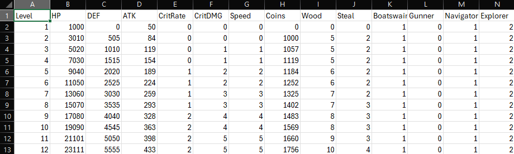
\includegraphics[width=5in]{annex/itemData1.png}

\paragraph{Json file}\hfill

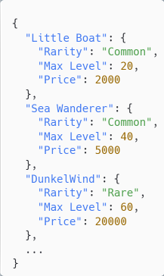
\includegraphics[width=2.5in]{annex/itemData2.png}





\newpage
\subsection*{2D Map}
\subsubsection*{Scratch}
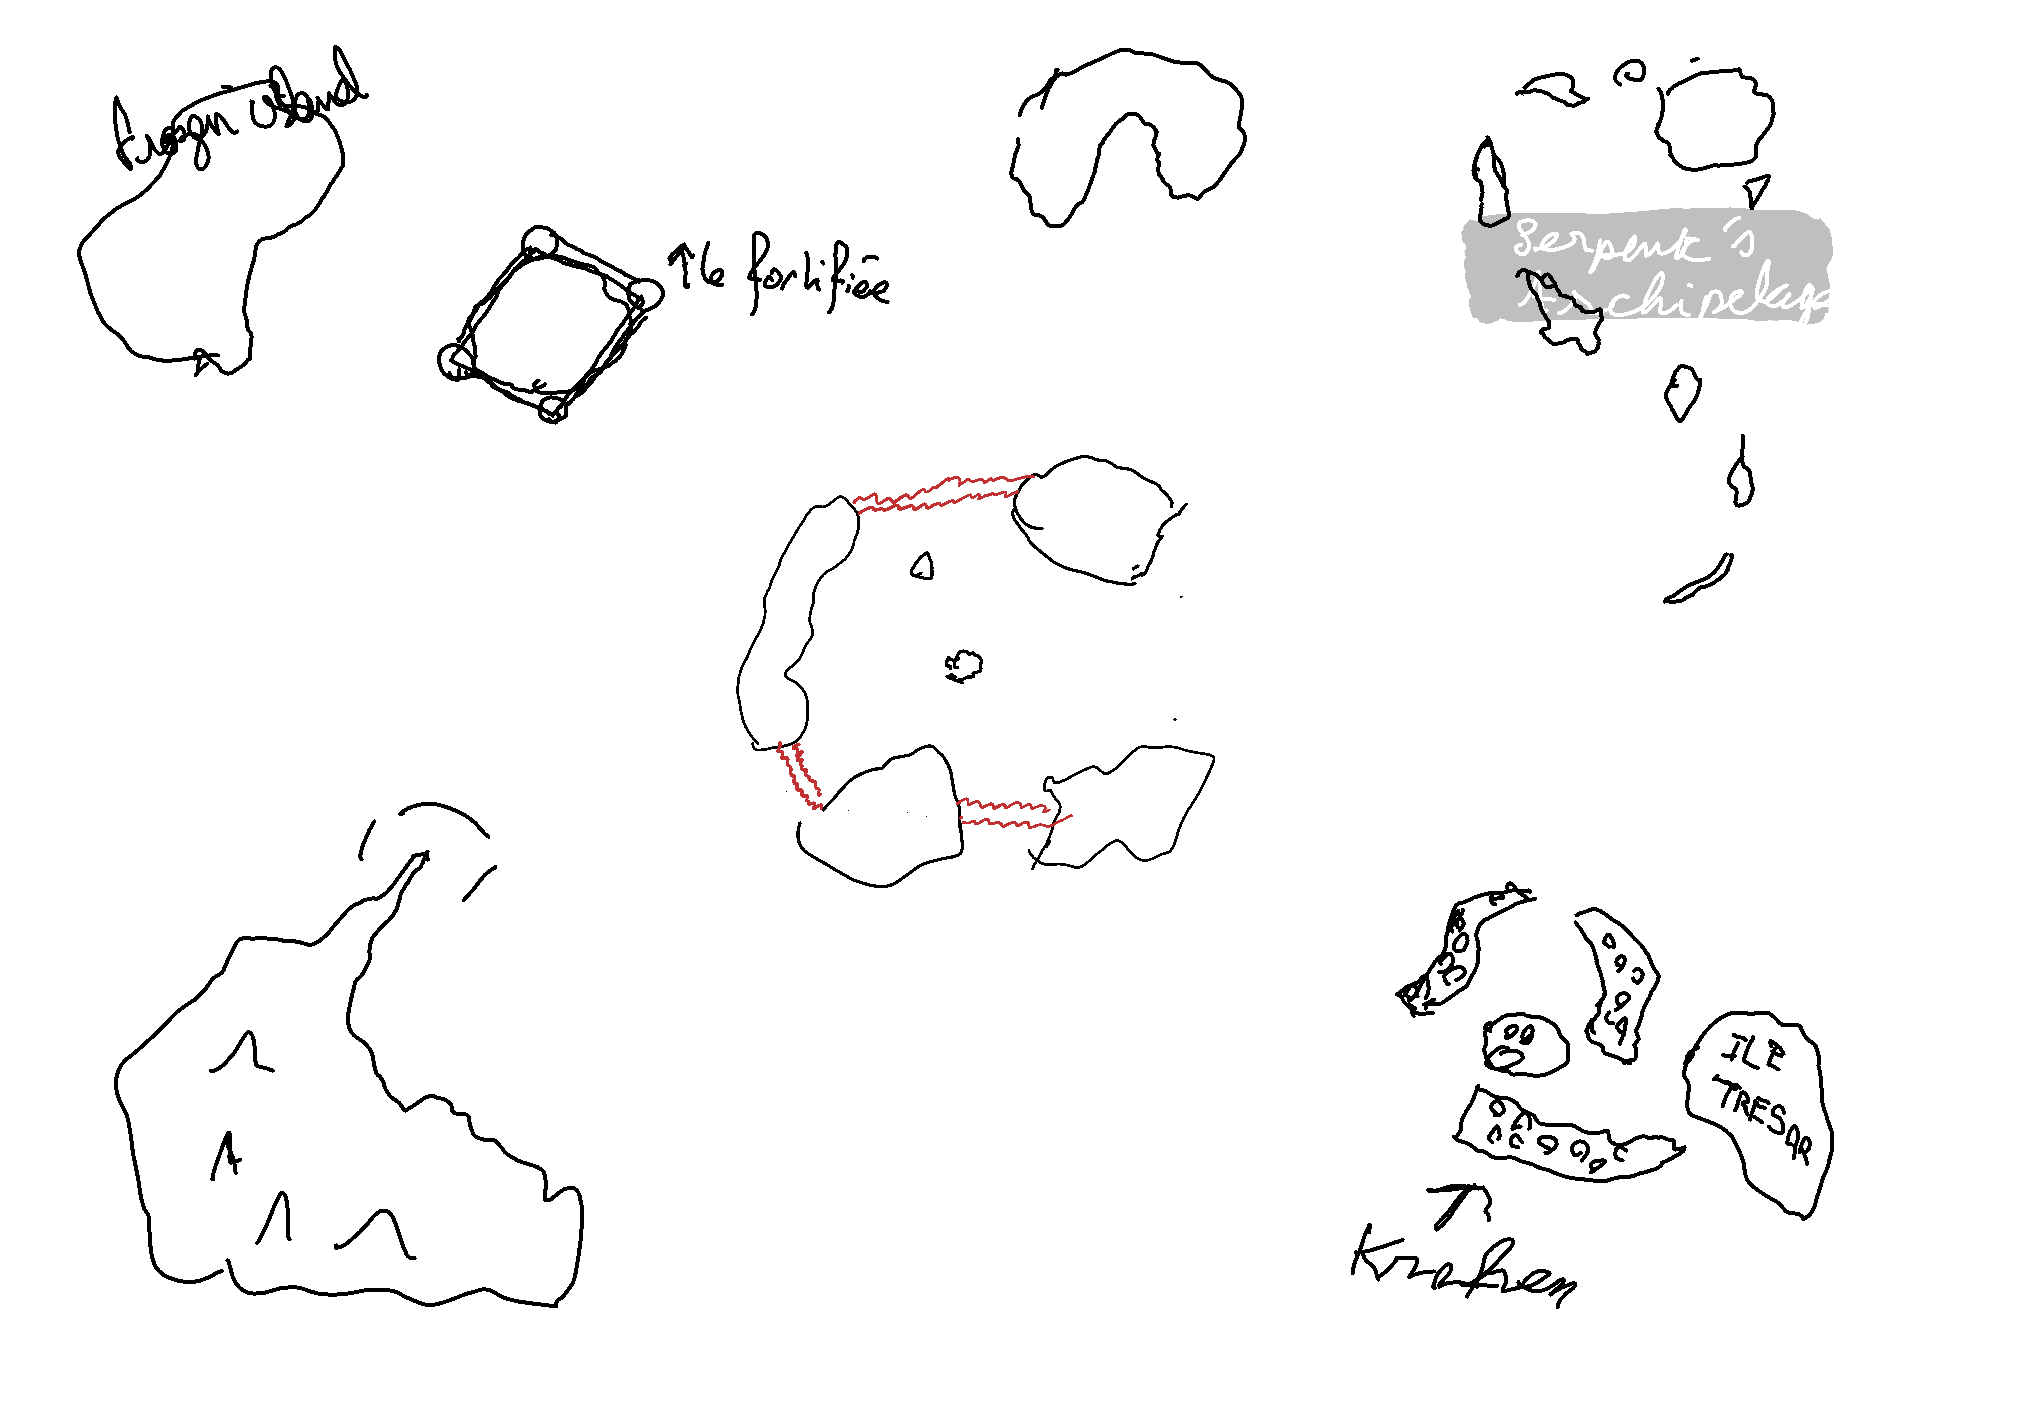
\includegraphics[width=5in]{annex/mapscratch.png}

\subsubsection*{Result}
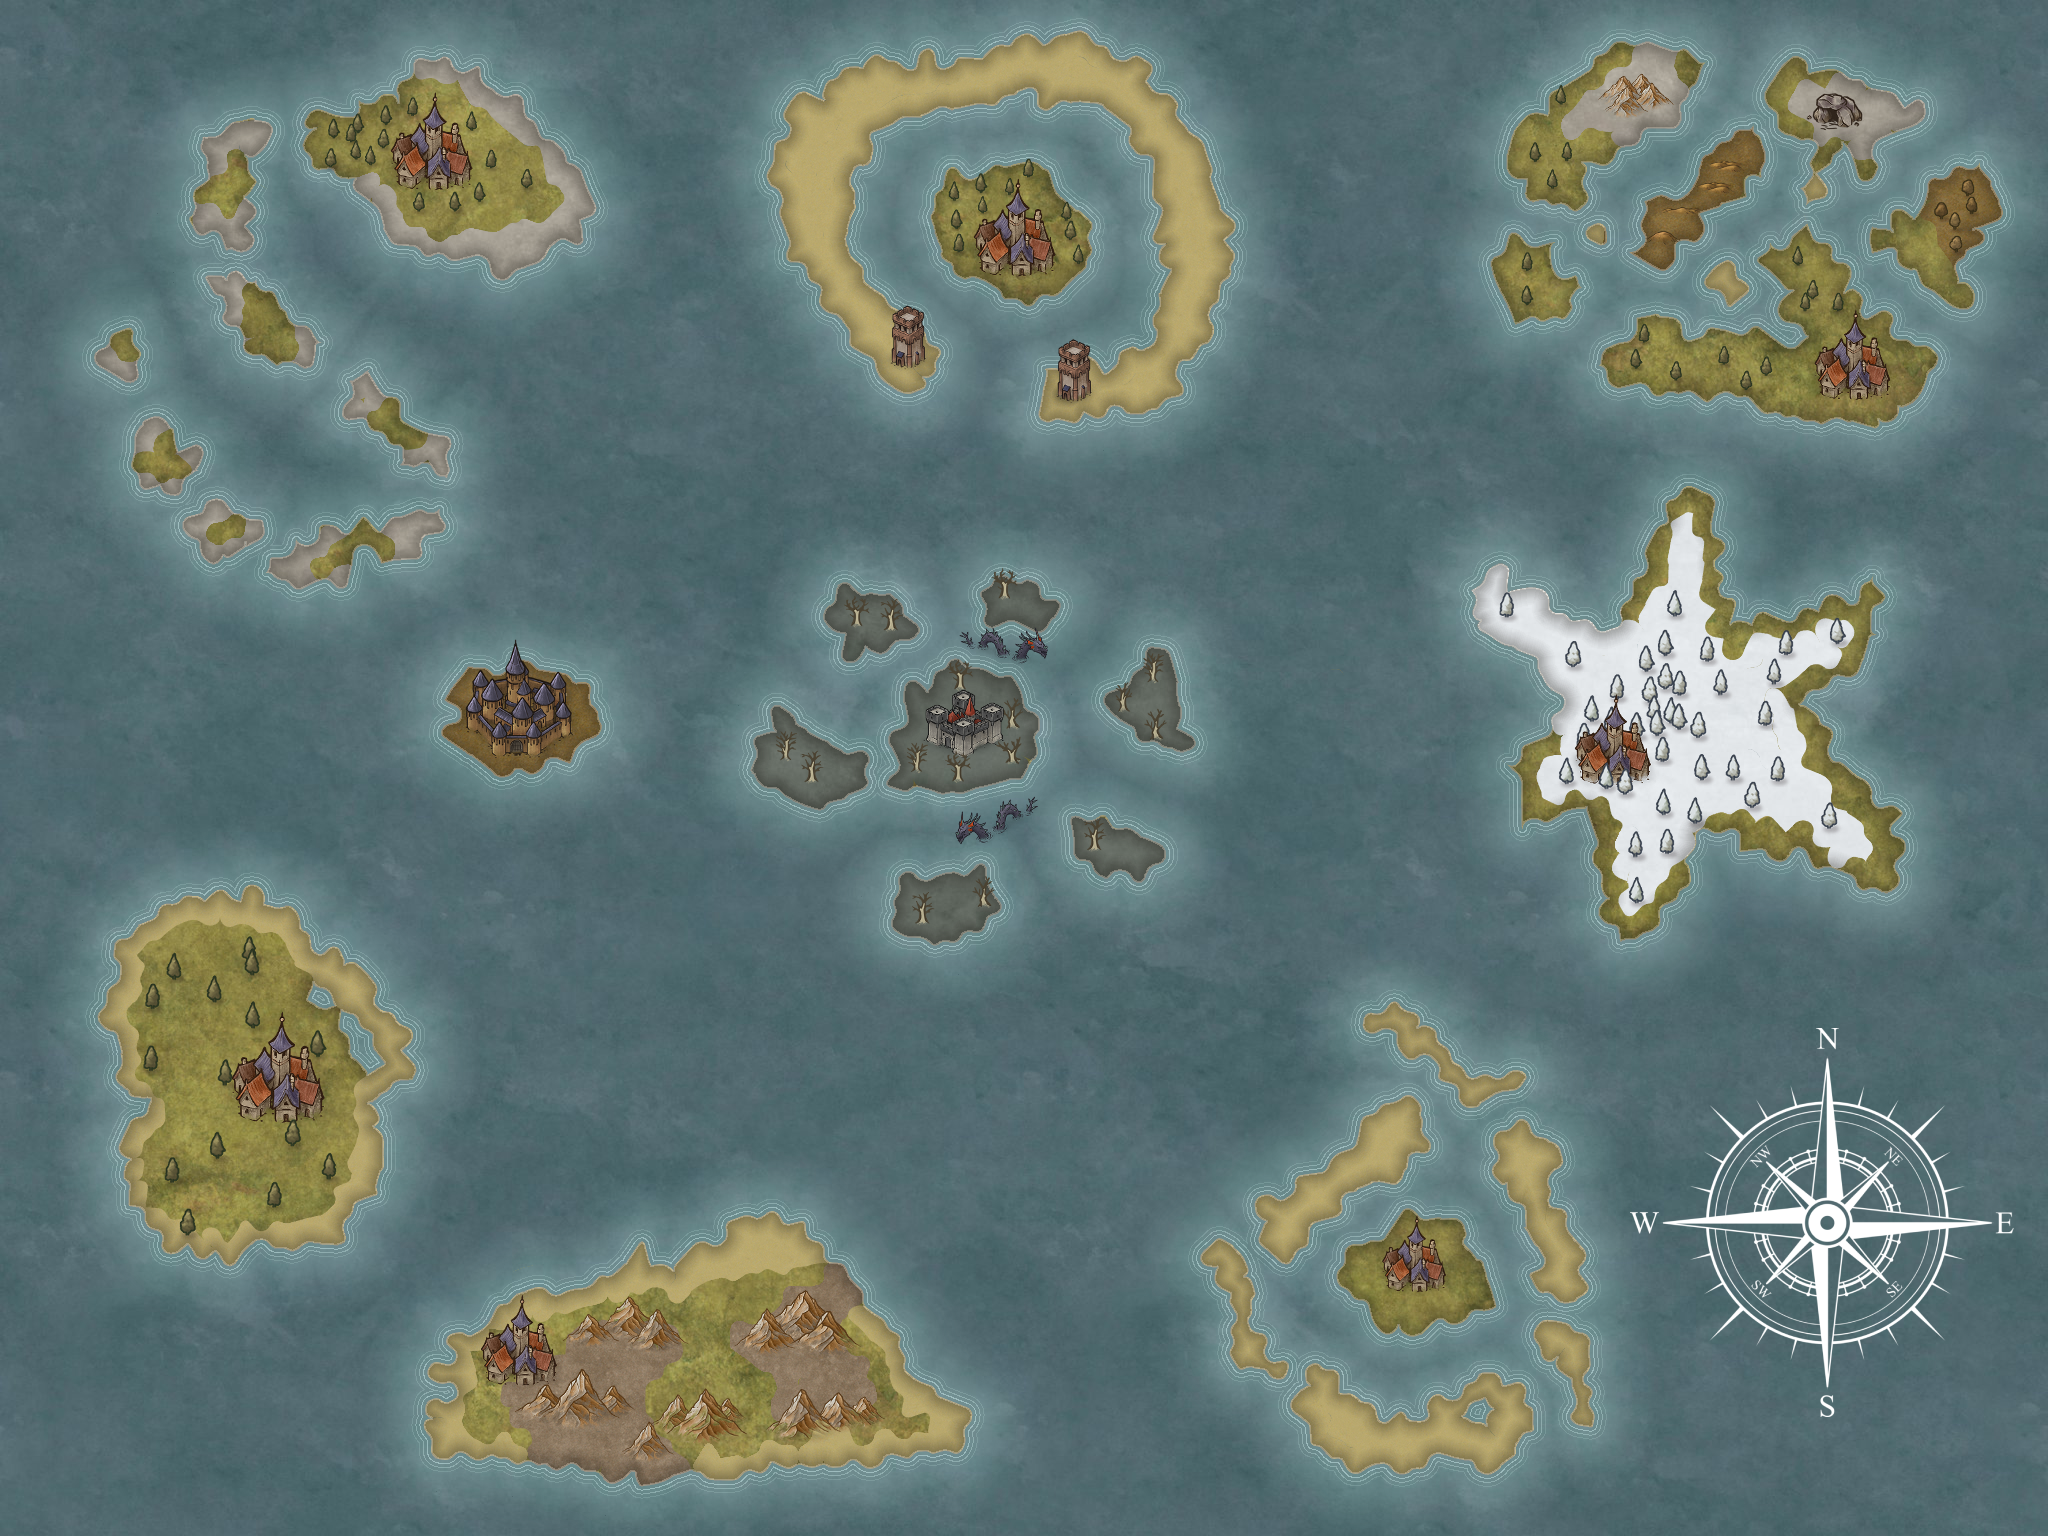
\includegraphics[width=5in]{annex/2dMap.png}





\newpage
\subsection*{3D Map}
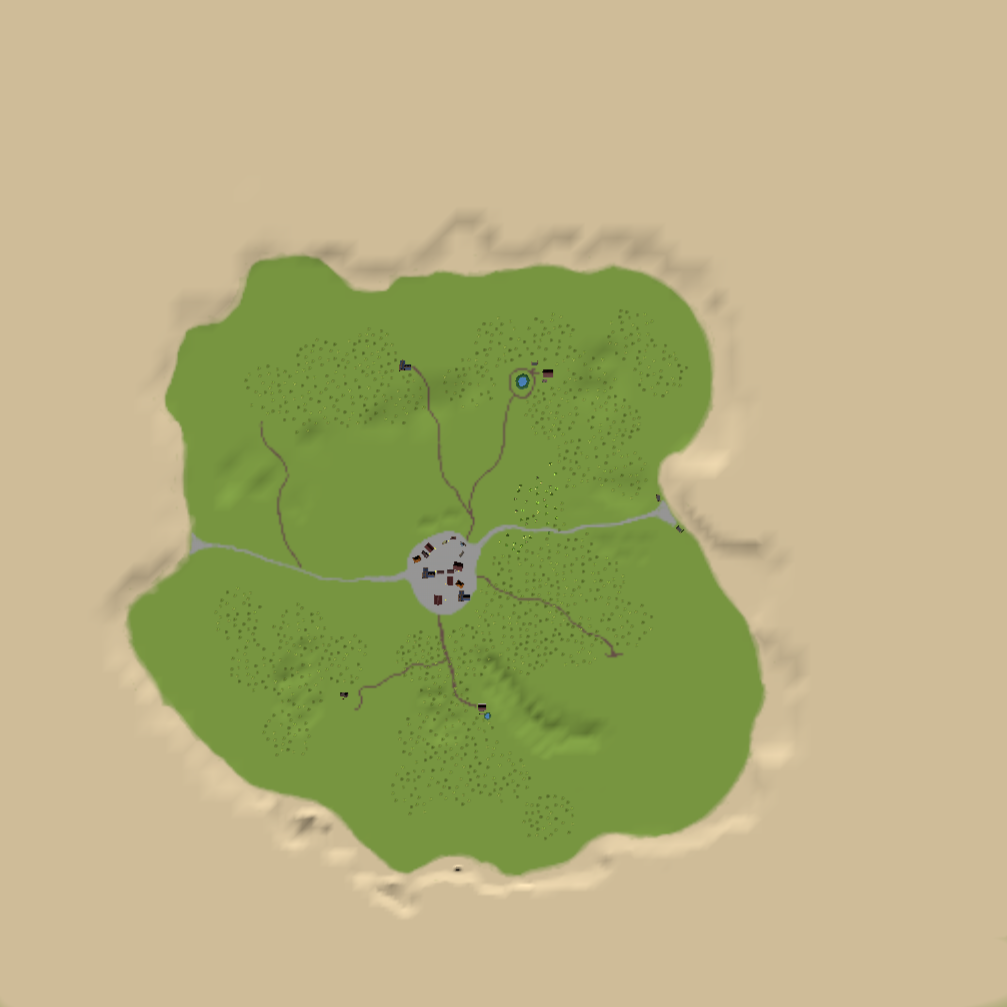
\includegraphics[width = 6in]{annex/3dMap1.png}\\
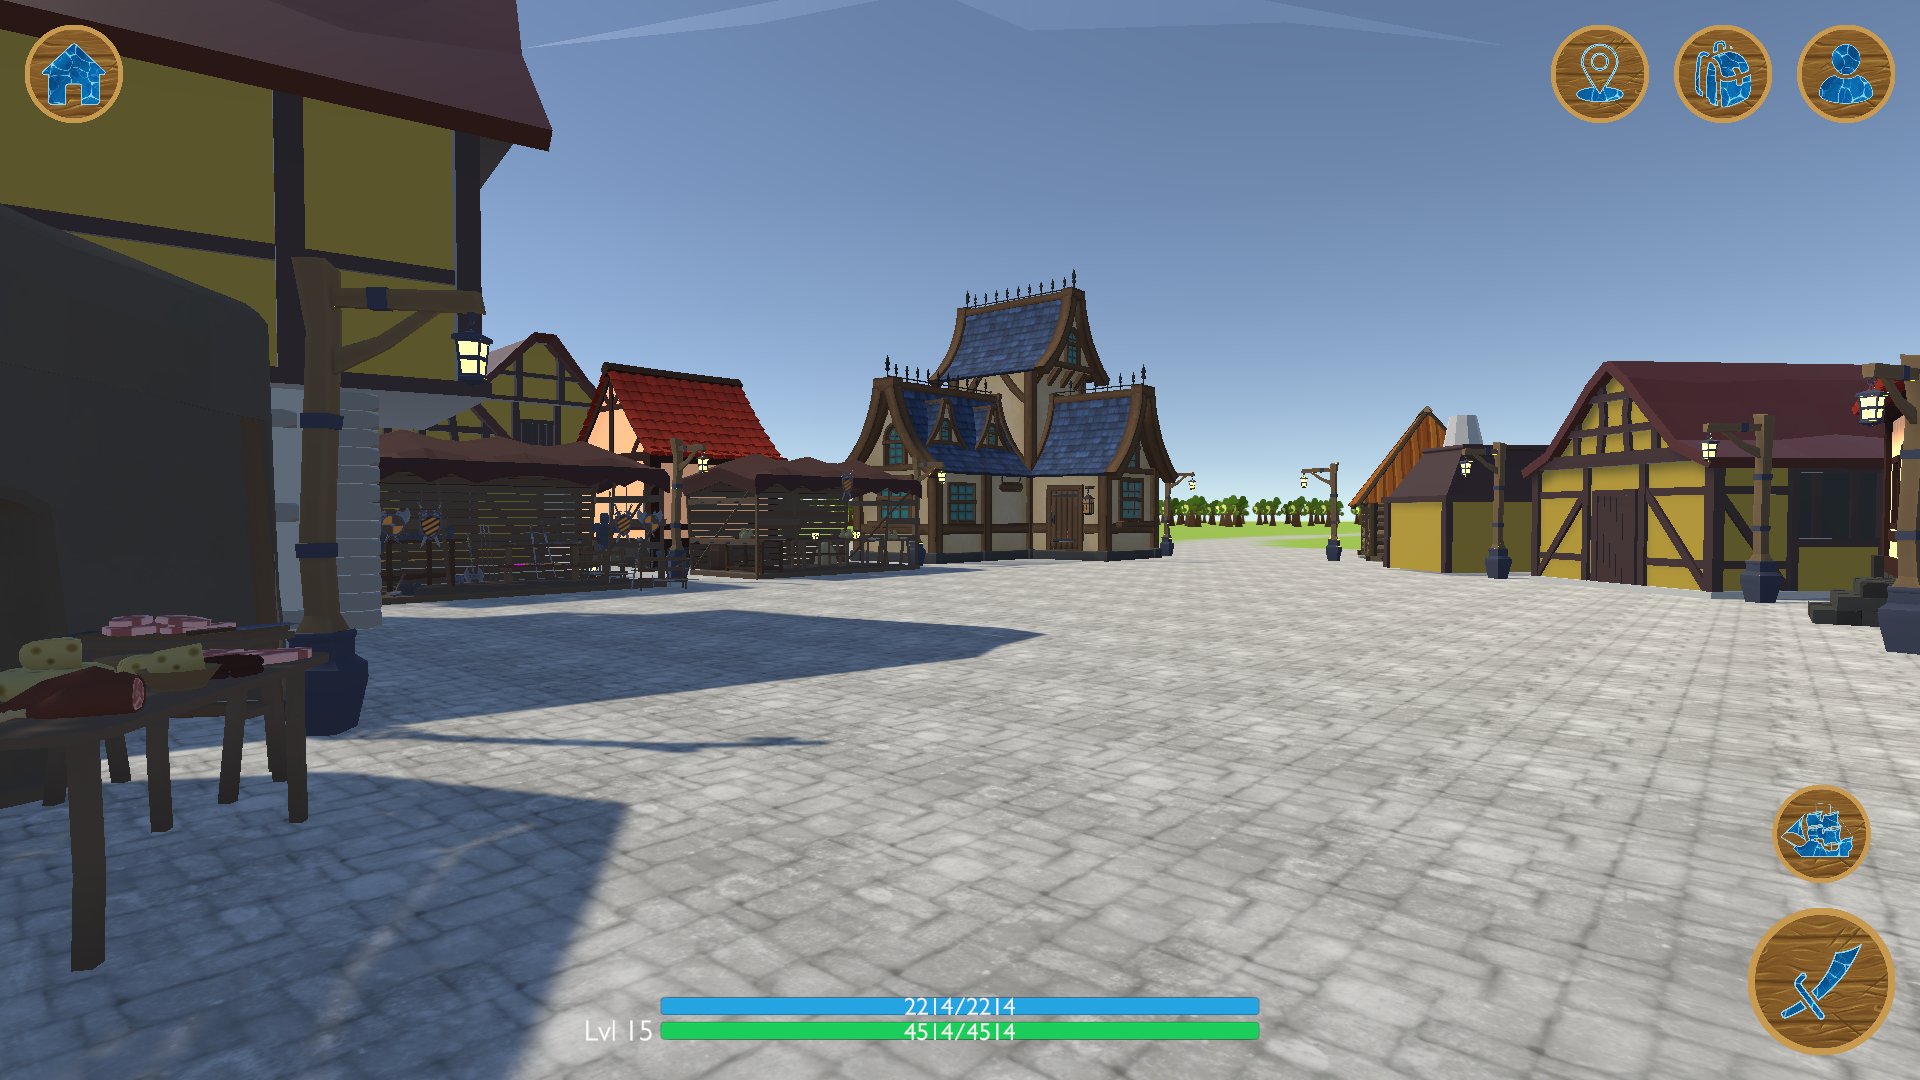
\includegraphics[width = 6in]{annex/3dMap2.png}





\newpage
\subsection*{Website}
https://dream-chasers.odoo.com\\
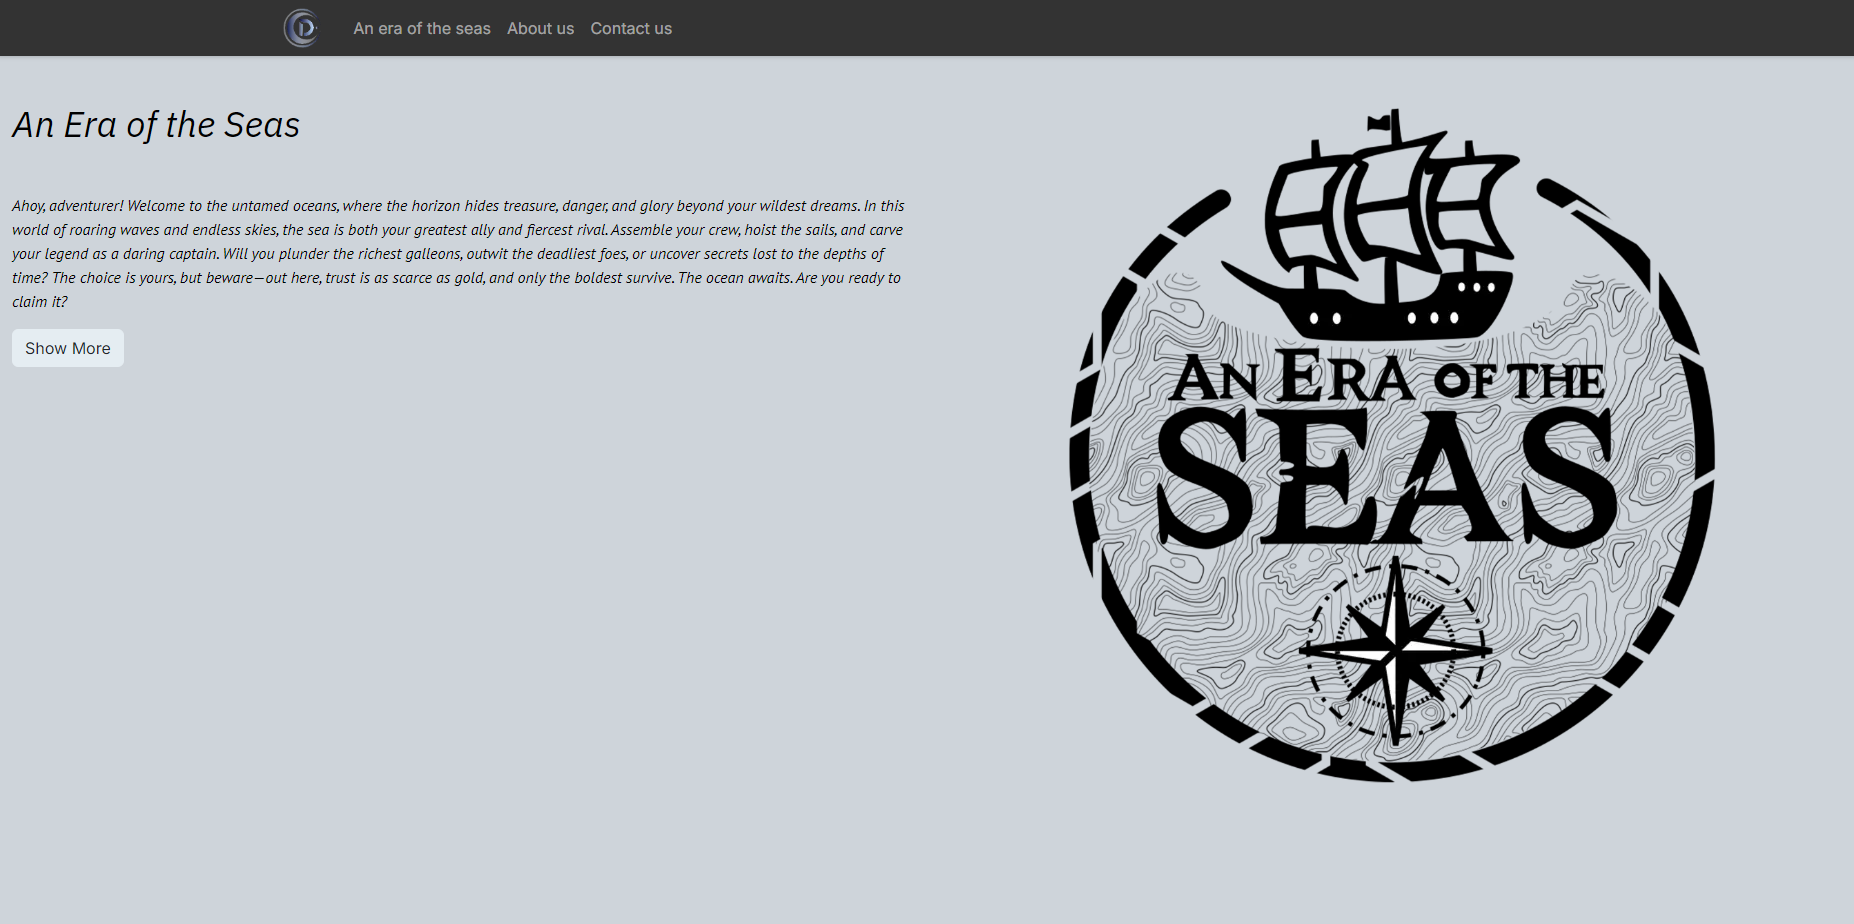
\includegraphics[width=6in]{annex/website1.png}\\

\includegraphics[width=6in]{annex/website2.png}\\

\includegraphics[width=6in]{annex/website3.png}





\newpage
\subsection*{Main Menu and UI}
\subsubsection*{Main Menu}
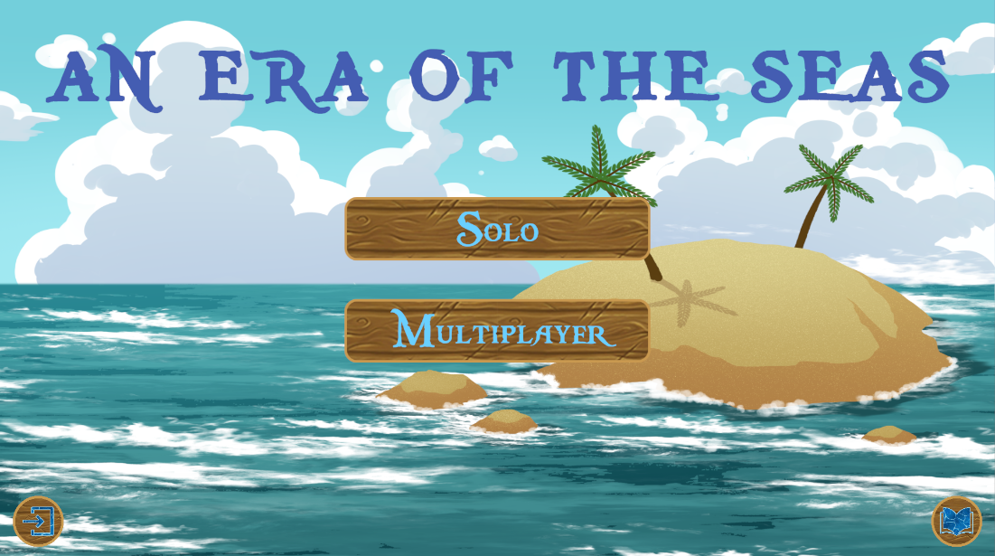
\includegraphics[width=6in]{annex/mainMenu.png}

\subsubsection*{Player interface}
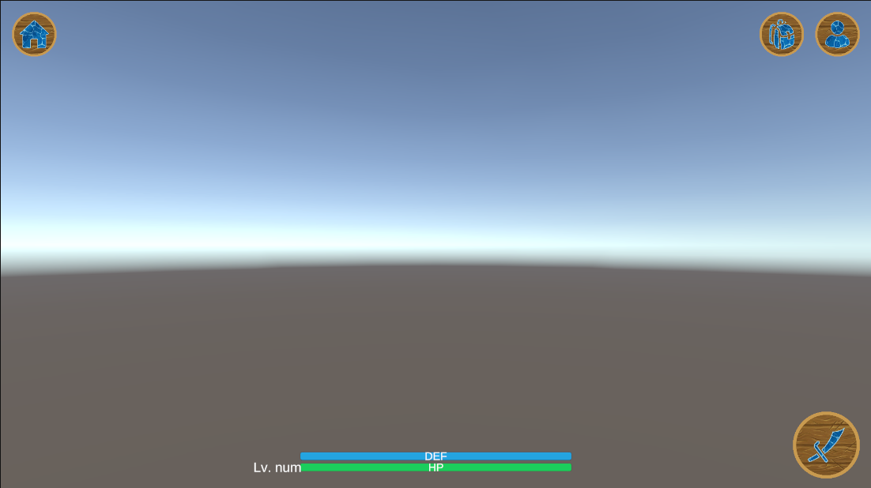
\includegraphics[width=6in]{annex/UI1.png}\\
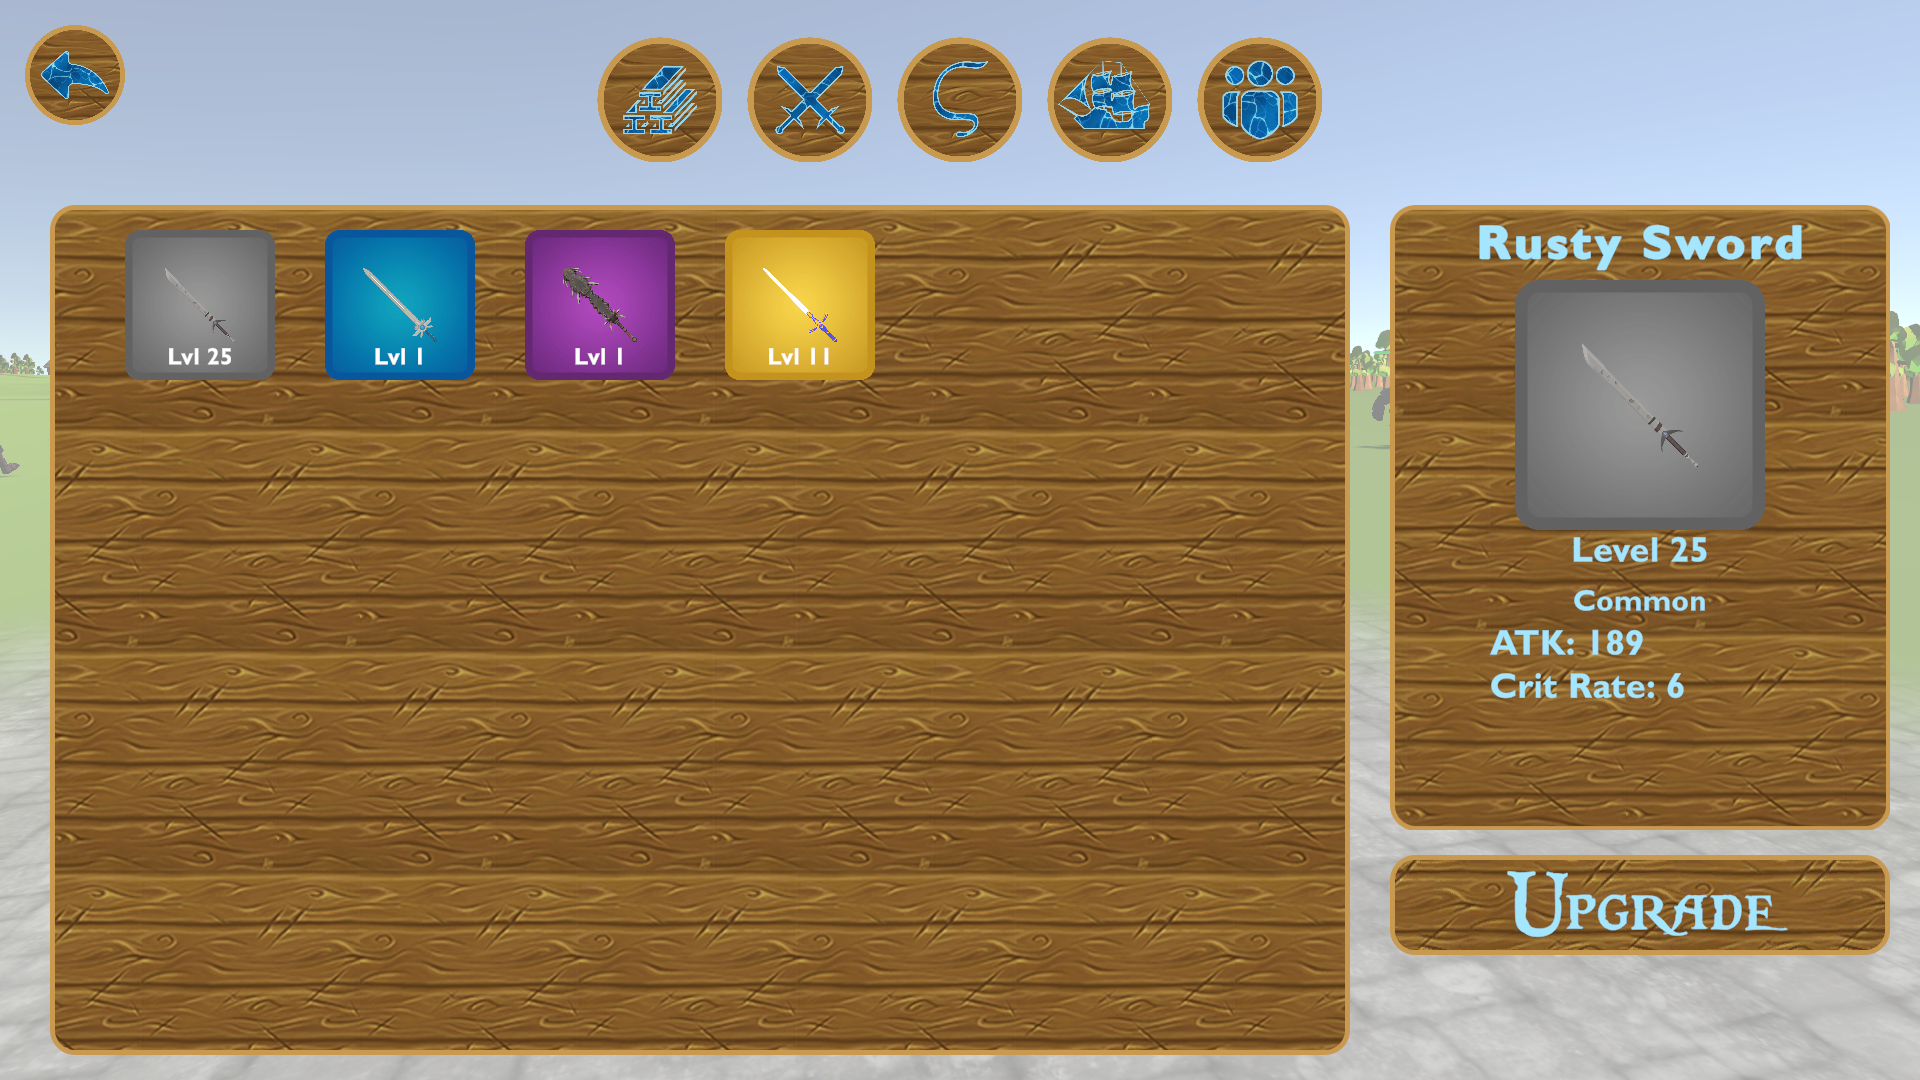
\includegraphics[width=6in]{annex/UI2.png}\\
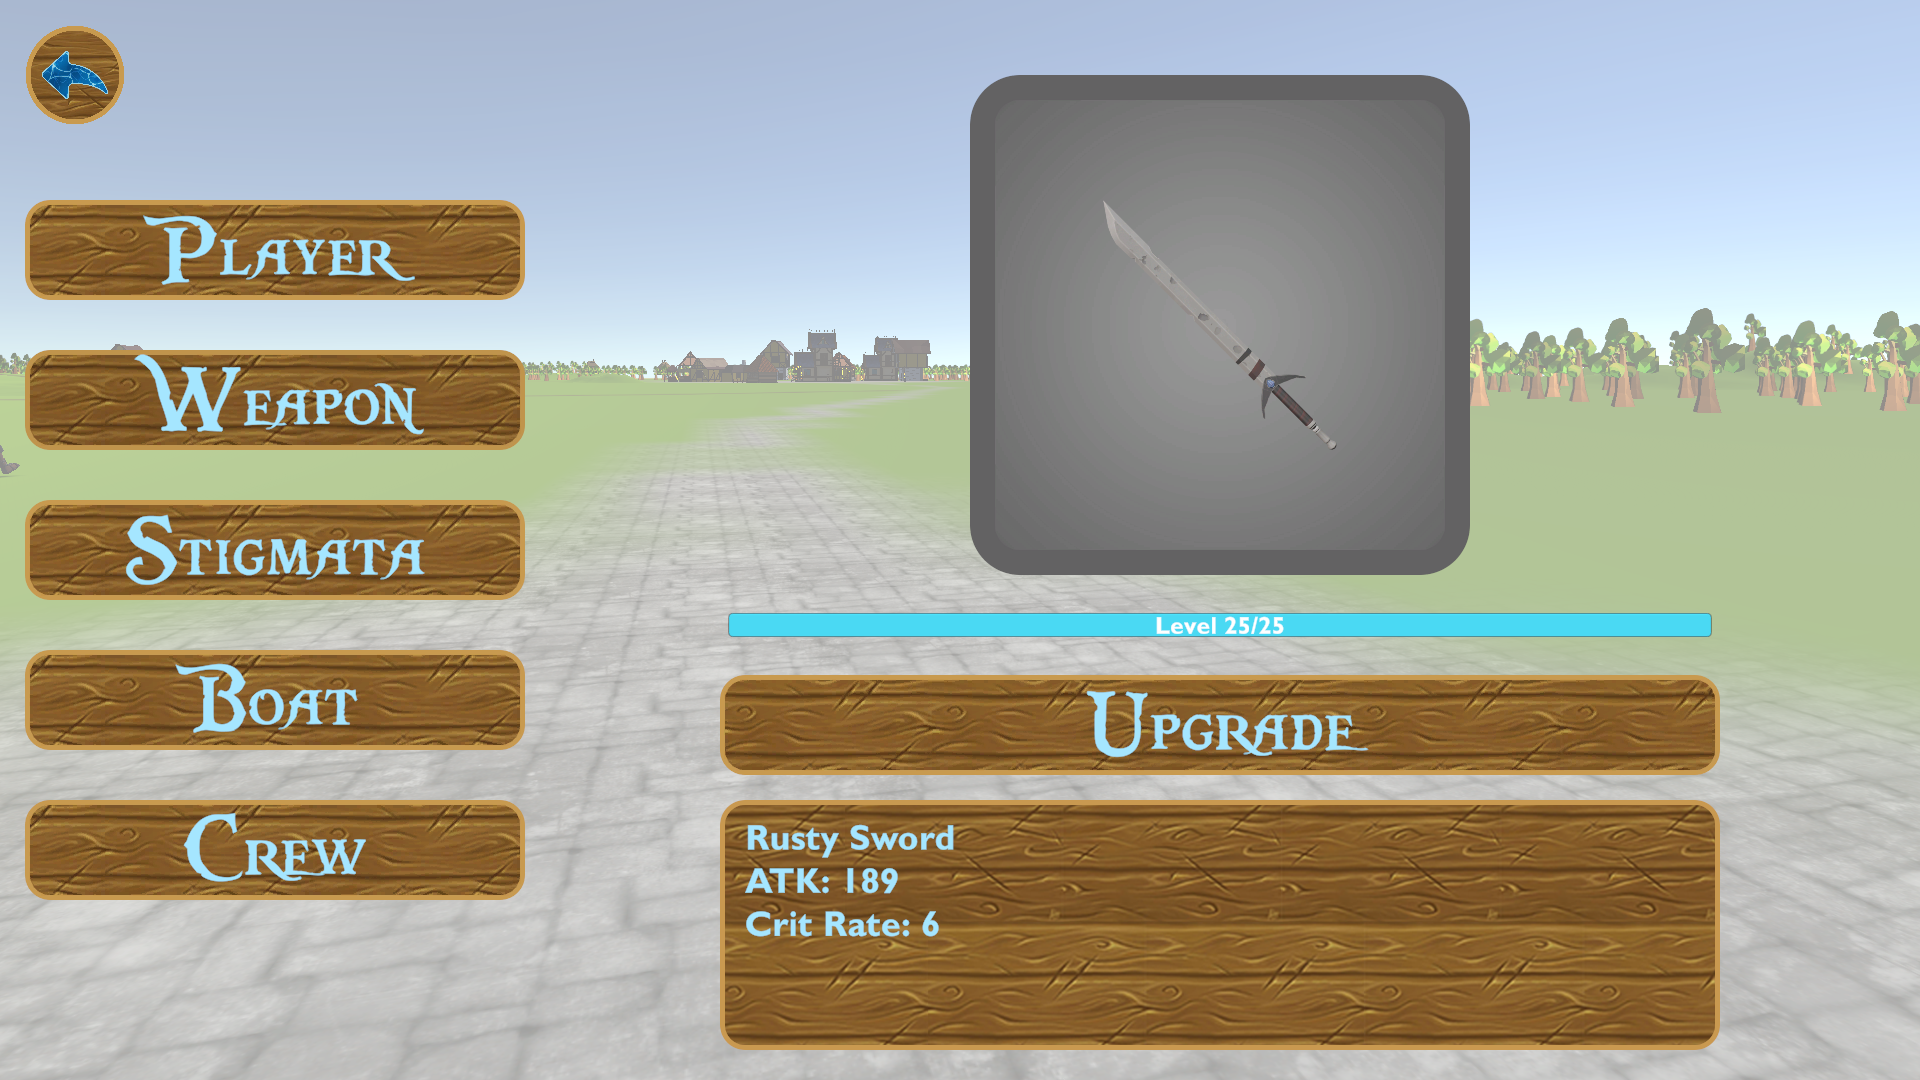
\includegraphics[width=6in]{annex/UI3.png}





\newpage
\subsection*{Water Simulation \& Boat Movements}
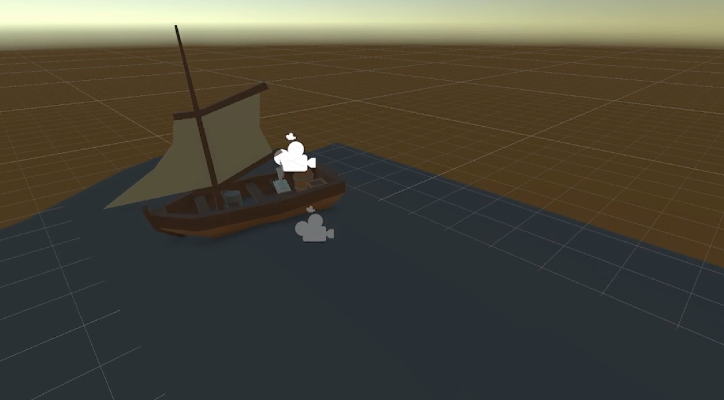
\includegraphics[width=6in]{annex/BoatMovement1.png}\\
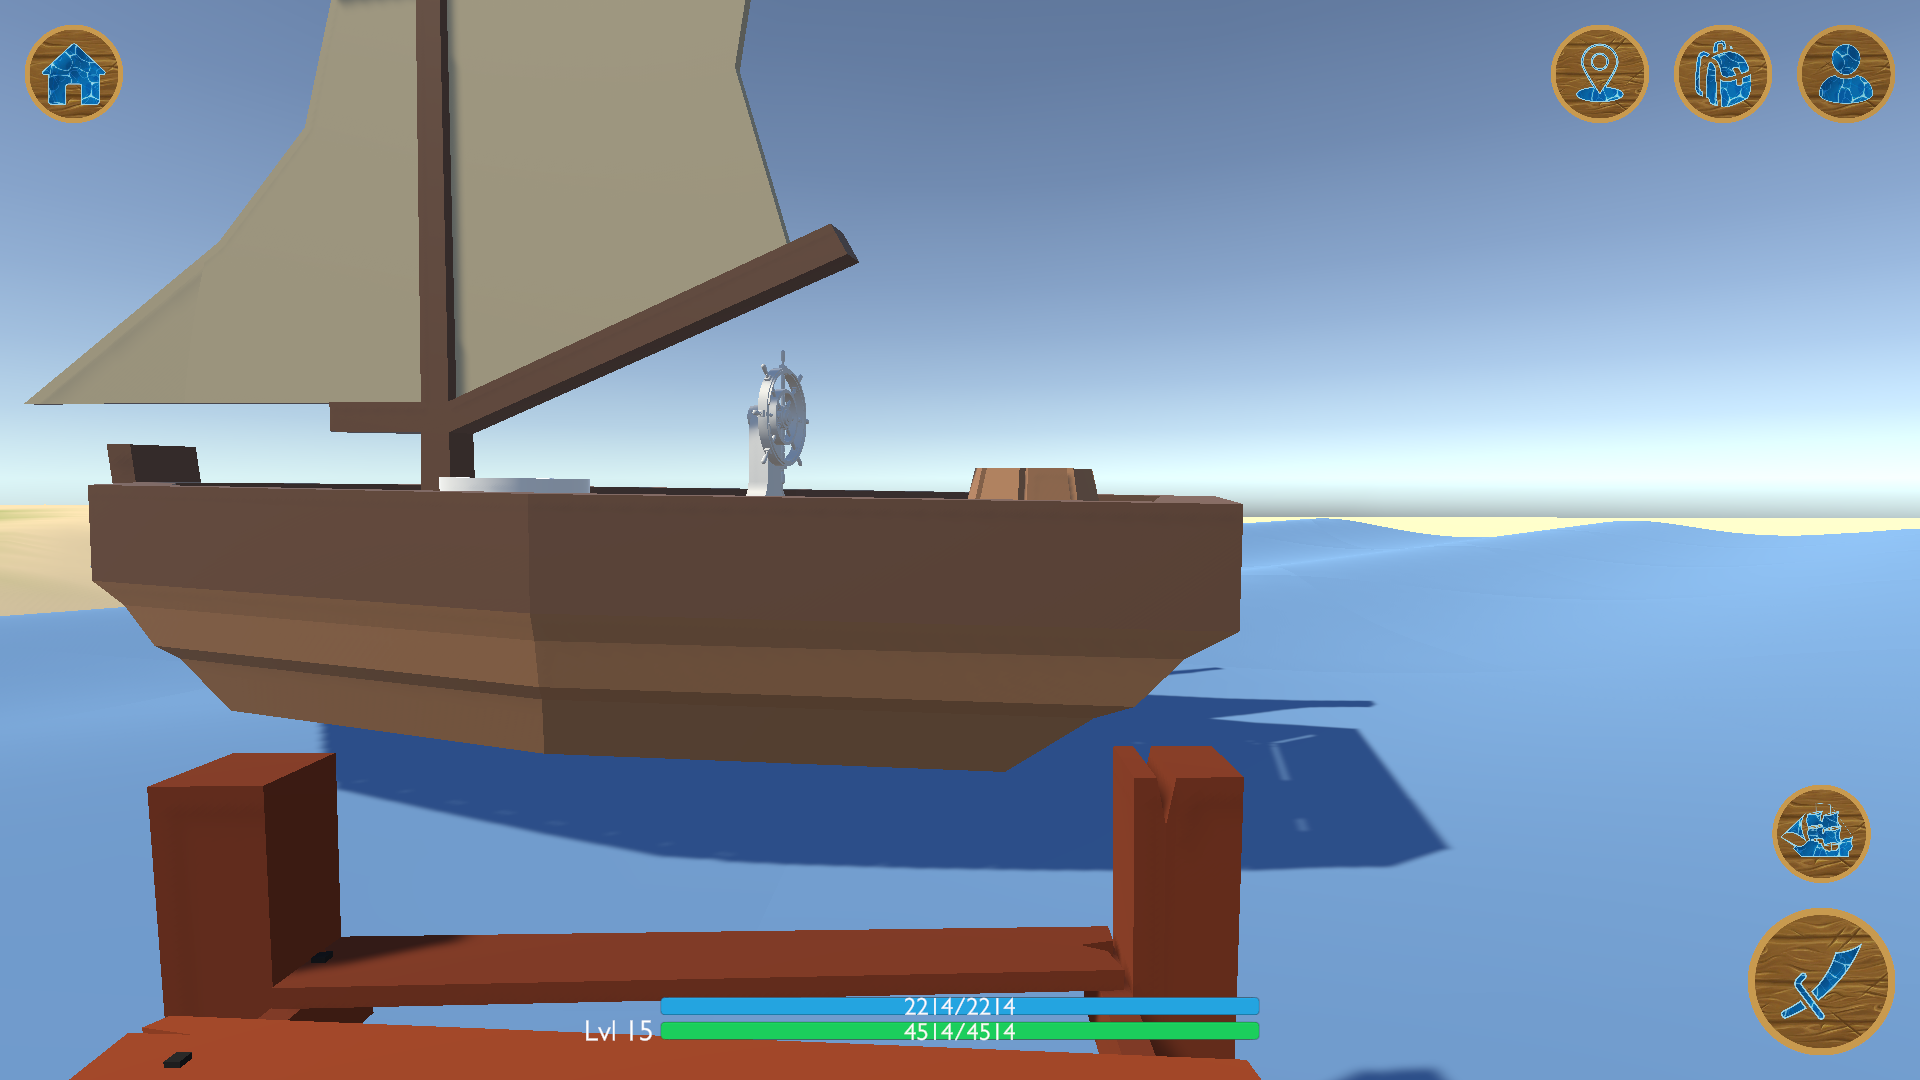
\includegraphics[width=6in]{annex/BoatMovement2.png}




\newpage
\subsection*{Animation}
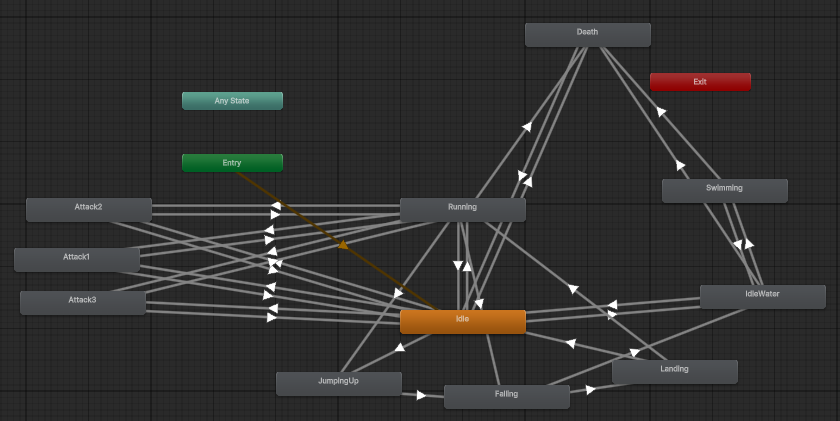
\includegraphics[width=6in]{annex/playeranimator.png}\\
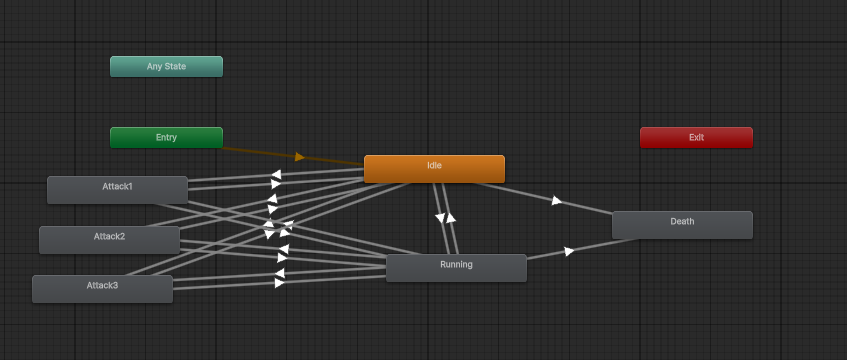
\includegraphics[width=6in]{annex/enemyanimator.png}





\newpage
\subsection*{Combat system}
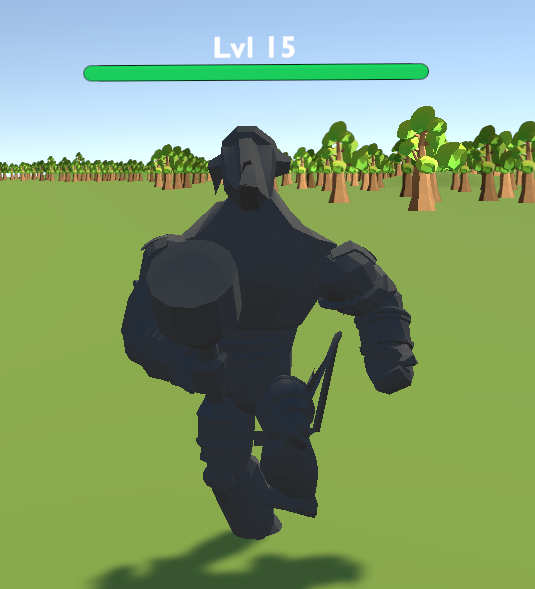
\includegraphics[width=5in]{annex/Combat1.png}\\
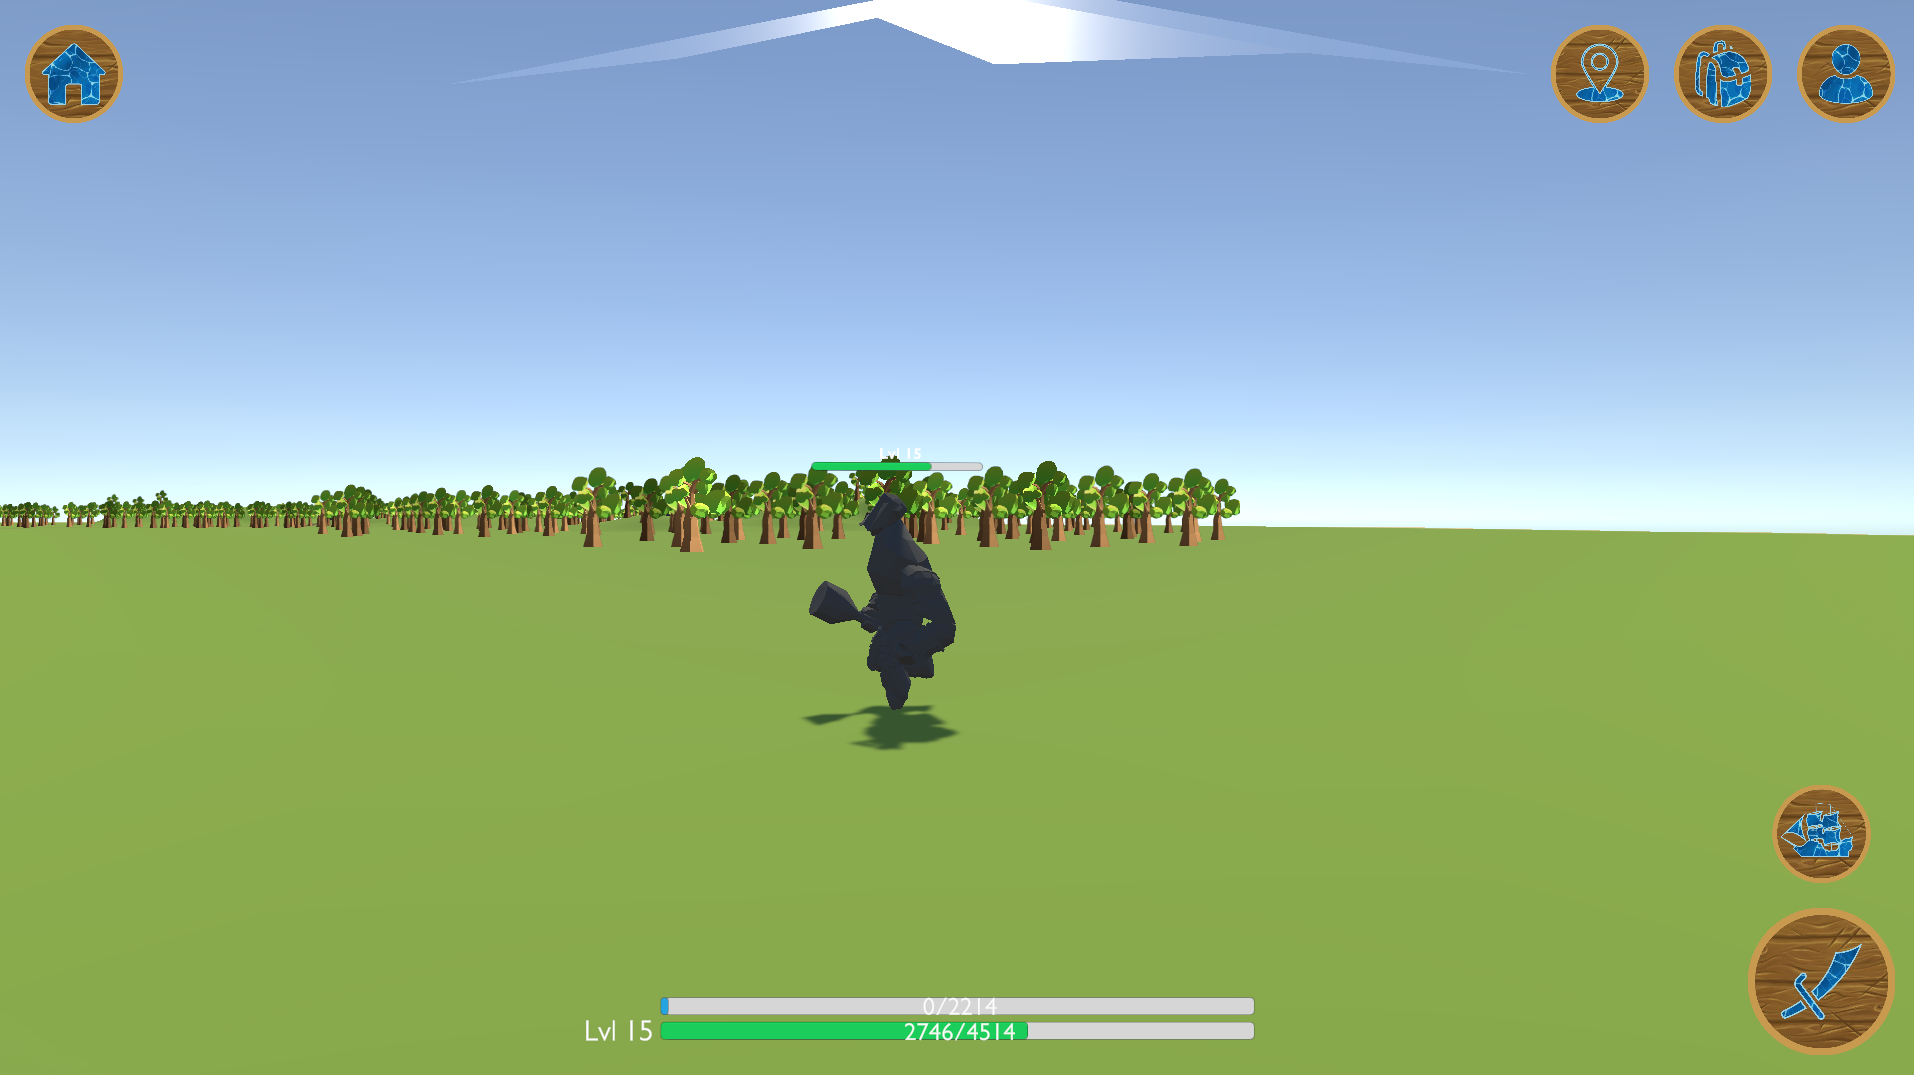
\includegraphics[width=6in]{annex/Combat2.png}





\end{document}